\documentclass{article}
\usepackage{placeins}
\usepackage{graphicx}
\usepackage{subcaption}
\usepackage{listings}
\usepackage{hyperref}
\usepackage{cleveref}
\usepackage{booktabs, siunitx}
\usepackage[svgnames,table]{xcolor}
\usepackage[utf8]{inputenc}
\usepackage[utf8]{inputenc}
\usepackage{geometry}

\geometry{
 a4paper,
 total={170mm,257mm},
 left=20mm,
 top=20mm,
 }
\graphicspath{ {./images/} }

\title{Assignment 1 Report}
\author{Tanat Tangun 630610737}
\date{August 2022}

\begin{document}
\maketitle

This report is about the result from using my implementation of the multi-layers perceptron
on Rust language to solve 2 problems given on 261456 - INTRO COMP INTEL FOR CPE class. 
If you are interested to know how I implement the multi-layers perceptron and trained a model to solve these problems
, you can see the source code for all models that have been shown in this report on my 
\href{https://github.com/RiwEZ/MLPOnRust}{Github repository}.

\section*{Flood Dataset}
\label{section:1}
\subsection*{Problem}
We want to predict water level at 7 hours ahead given station 1 and station 2 
data at present, 1 hour before, 2 hours before, and 3 hours before. 
\begin{figure}[ht]
	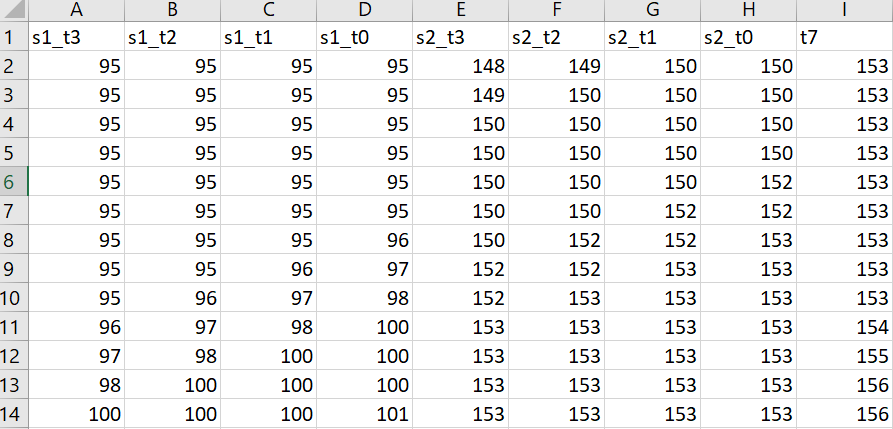
\includegraphics[width=\textwidth]{flood_data}
	\caption{Examples of given data
		where s1\_t3 is water level from 3 hours before at station 1, and so on.
		t7 is water level at 7 hours ahead.}
	\label{fig:1}
\end{figure}

\subsection*{Parameters Setting}
\begin{itemize}
	\item All nodes use $sigmoid$ as an activation function except output node that use $linear$ function.
	\item Weights are random number that is in range $[-1, 1]$
	\item Each layer's bias is $1$
	\item Use MSE (Mean Squared Error) as a loss function.
\end{itemize}

\subsection*{Training}
Use 10\% cross-validation, and preprocess our data by using training set $mean$ 
and $std$ to standardize (For each data point $x$ we calculate new 
$x' = \frac{x - mean}{std}$) both training set and validation set before 
training with SGD (Stochastic Gradient Descent) algorithm. 
Then, we train each cross-validation set for $1000$ epochs.

We will create one base model that should perform good enough 
and create a variations base on that model. For this problem we will introduce these variations
i.e. train with no \emph{momentum}, train with smaller \emph{learning rate}, train with no data preprocessing 
and add more layers or hidden nodes to see that if we introduce those variations, 
will the model perform better, converge faster, or have no improvement at all?

\subsection*{Training Result}
\subsubsection*{Flood-8-4-1}
Our base model that contains only 8 input nodes, 1 hidden layer with 4 nodes, and 1 output node train with $lr = 0.01$ and $momentum = 0.01$.
The training process takes about $56$ seconds. Below are the graphs we get from training this model. 
\begin{figure}[ht]
	\begin{subfigure}{\textwidth}
		\centering
		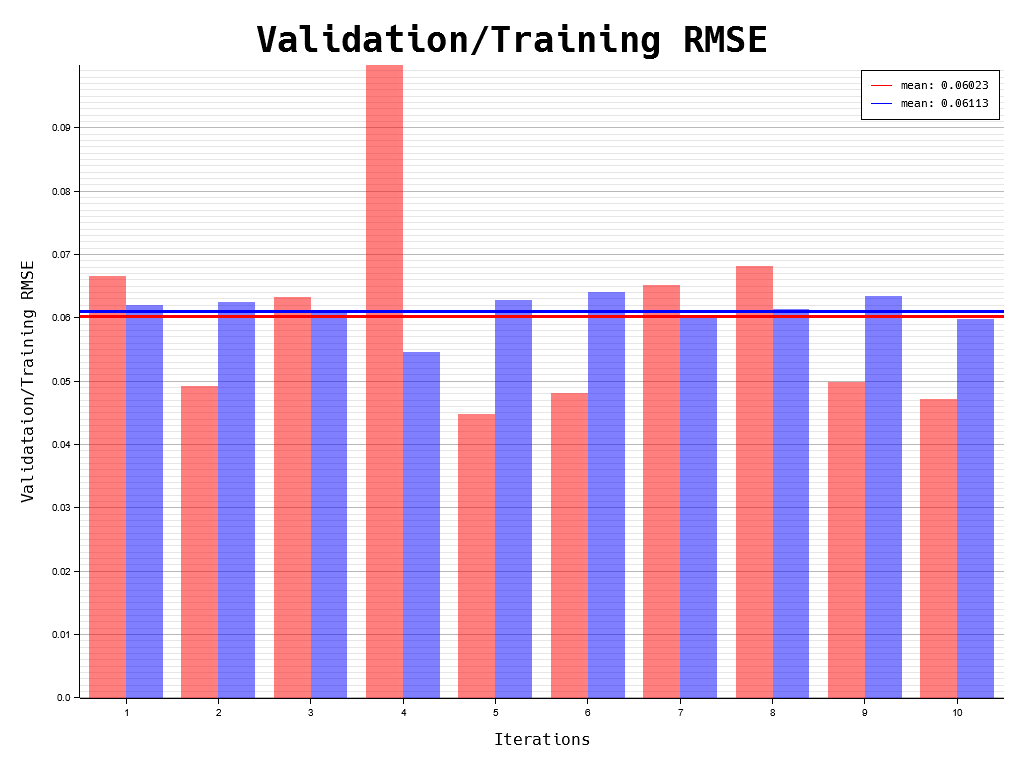
\includegraphics[scale=0.3]{flood-8-4-1/cv_l}
		\caption{Each iteration training (blue) and validation (red) RMSE at last epoch}
		\label{fig:2a}
	\end{subfigure}
	\begin{subfigure}{\textwidth}
		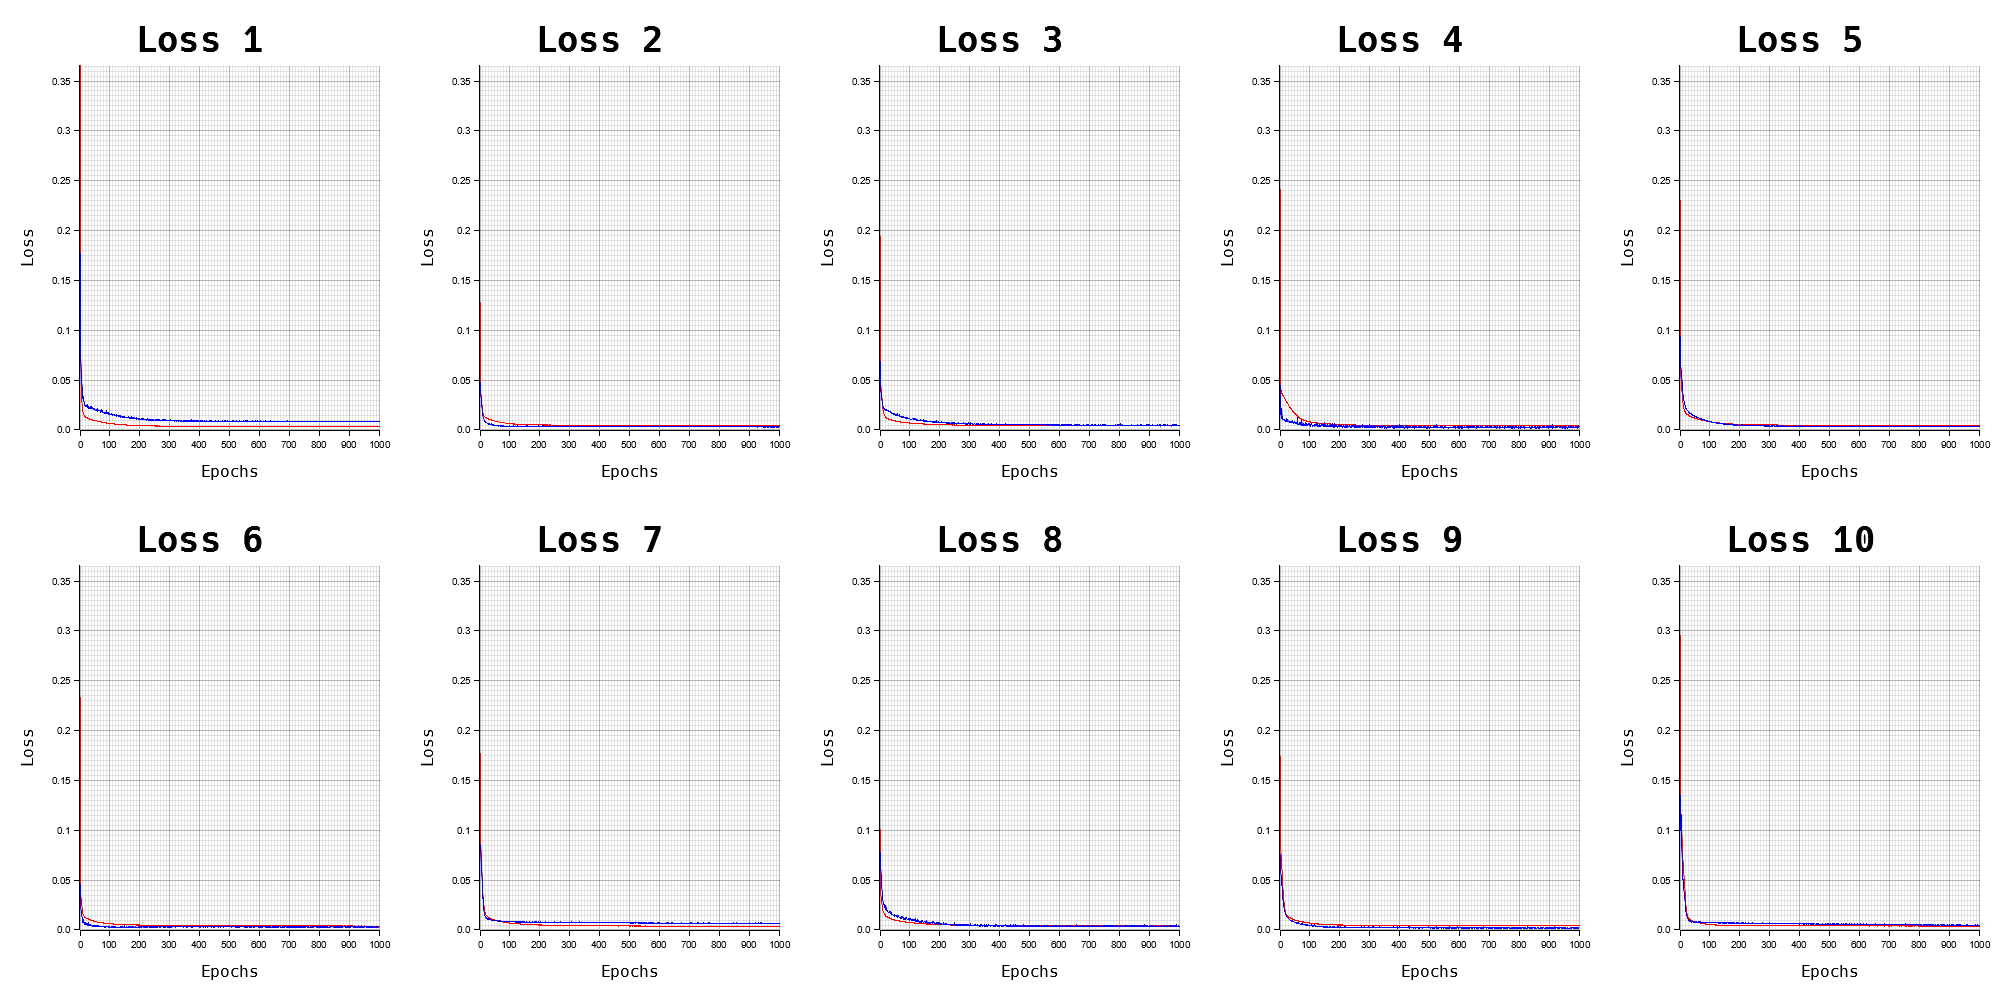
\includegraphics[width=\textwidth]{flood-8-4-1/loss}
		\caption{Each iteration training MSE (blue) and validation MSE (red) at each epoch.}
		\label{fig:2b}
	\end{subfigure}
	\caption{Training result of Flood-8-4-1.}
	\label{fig:2}
\end{figure}
\FloatBarrier

\newpage
\subsubsection*{Flood-8-4-1 with no momentum}
Same base model but train with $lr = 0.01$ and $momentum = 0$.
The training process takes about $56$ seconds.
Below are the graphs we get from training this model. 
\begin{figure}[ht]
	\begin{subfigure}{\textwidth}
		\centering
		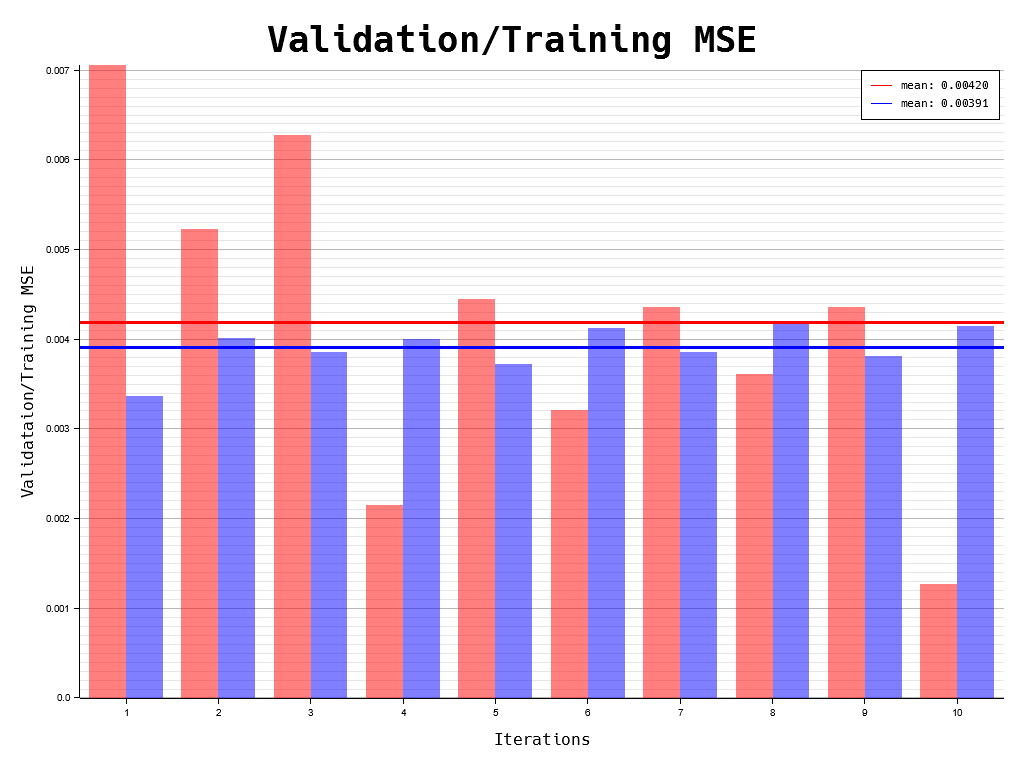
\includegraphics[scale=0.3]{flood-8-4-1_2/cv_l}
		\caption{Each iteration training (blue) and validation (red) RMSE at last epoch}
		\label{fig:3a}
	\end{subfigure}
	\begin{subfigure}{\textwidth}
		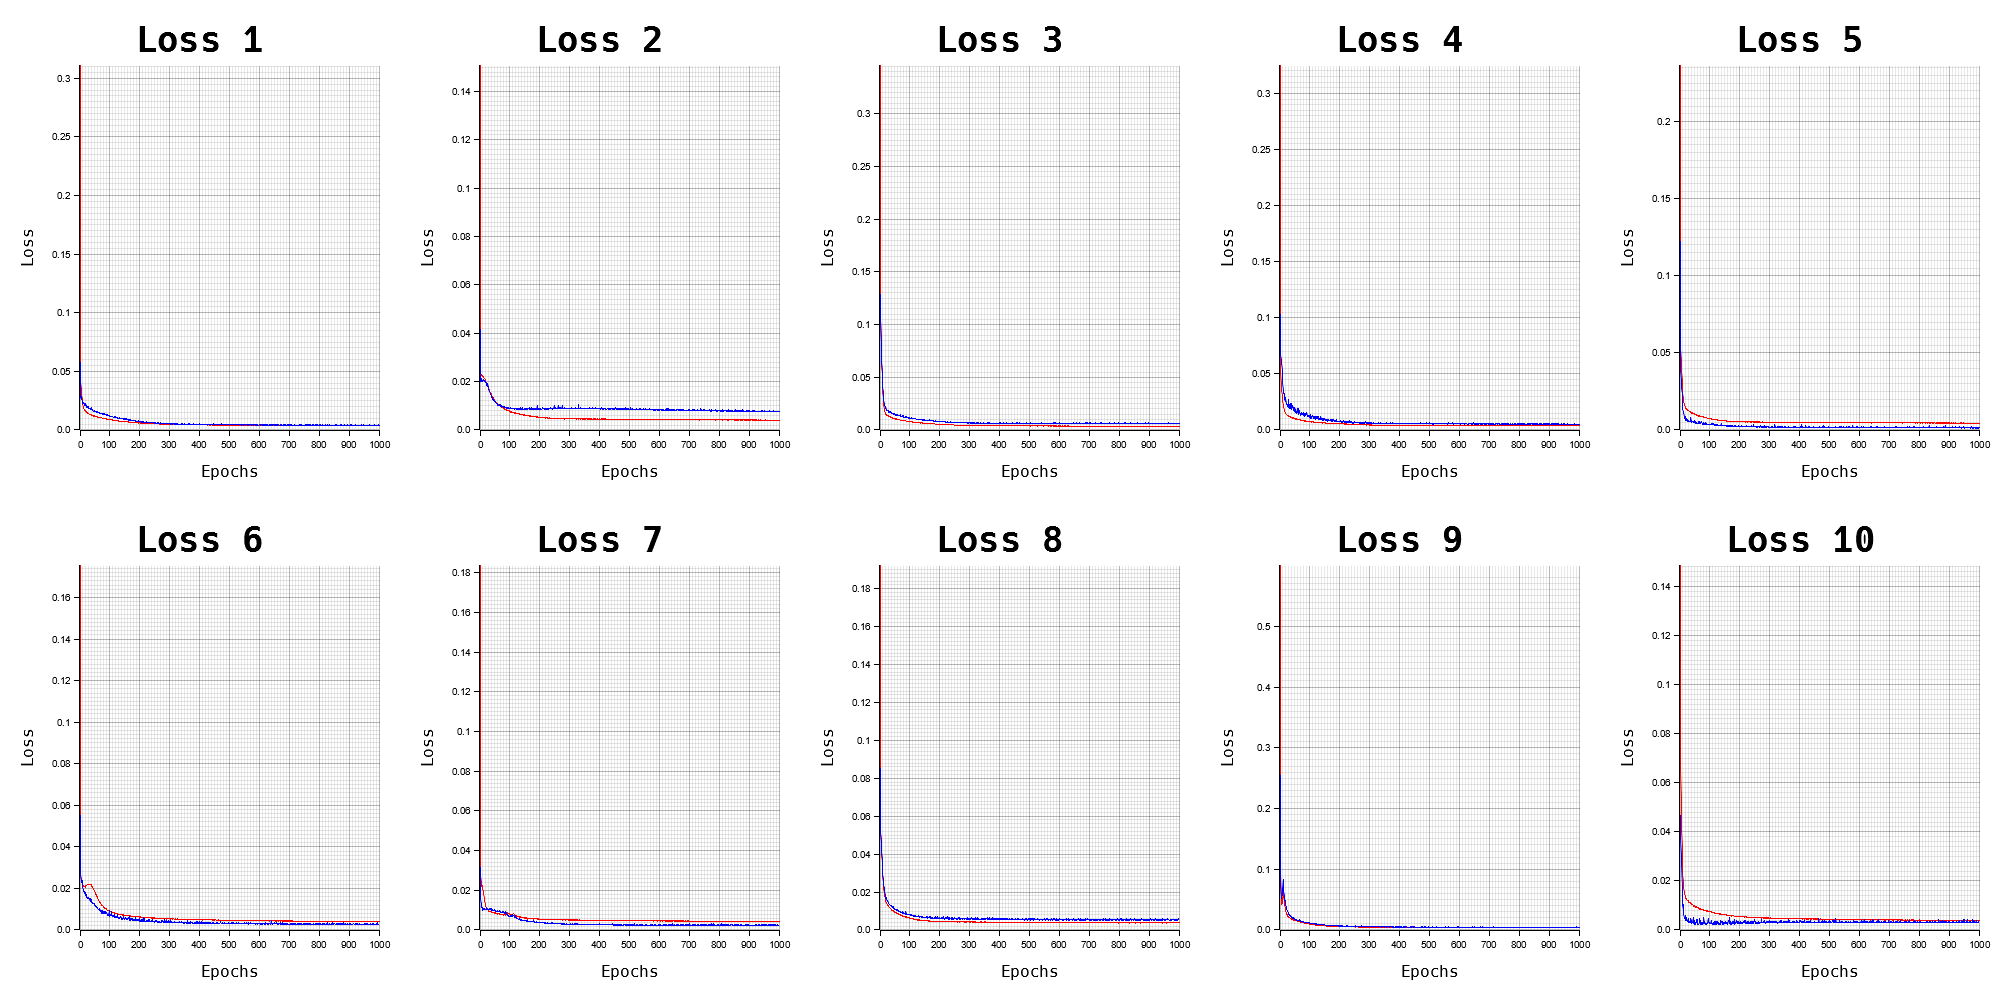
\includegraphics[width=\textwidth]{flood-8-4-1_2/loss}
		\caption{Each iteration training MSE (blue) and validation MSE (red) at each epoch.}
		\label{fig:3b}
	\end{subfigure}
	\caption{Training result of Flood-8-4-1 with no momentum.}
	\label{fig:3}
\end{figure}
\FloatBarrier

\newpage
\subsubsection*{Flood-8-4-1 with small learning rate}
Same base model but train with $lr = 0.0001$ and $momentum = 0.01$.
The training process takes about $56$ seconds.
Below are the graphs we get from training this model. 
\begin{figure}[ht]
	\begin{subfigure}{\textwidth}
		\centering
		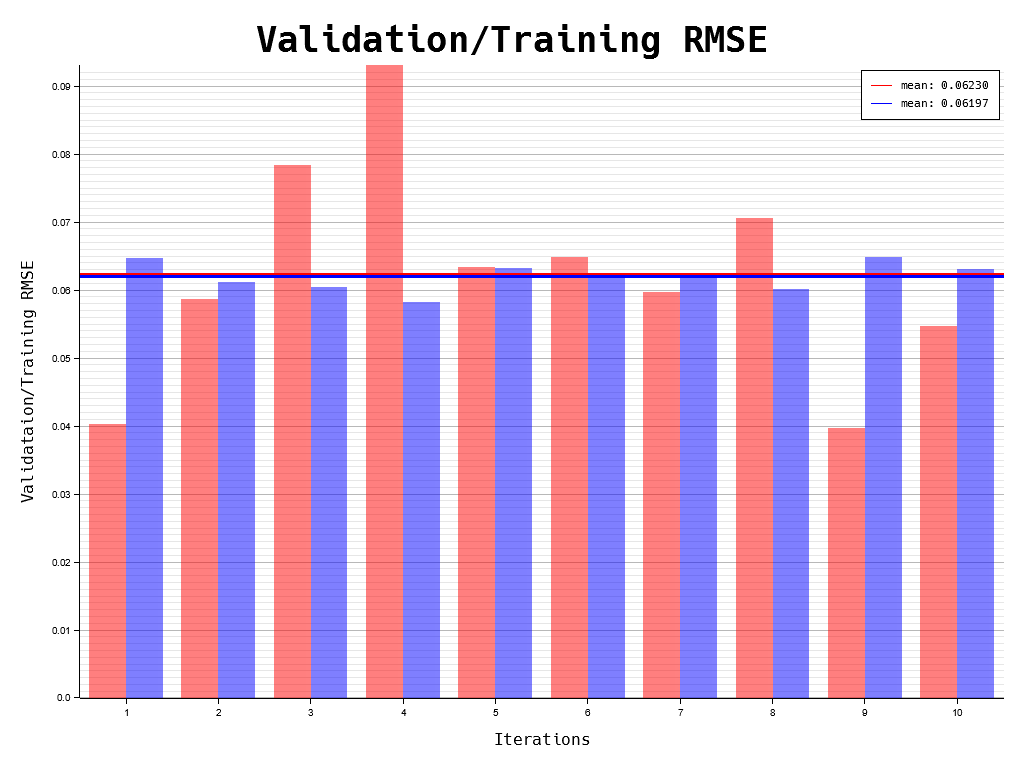
\includegraphics[scale=0.3]{flood-8-4-1_3/cv_l}
		\caption{Each iteration training (blue) and validation (red) RMSE at last epoch}
		\label{fig:4a}
	\end{subfigure}
	\begin{subfigure}{\textwidth}
		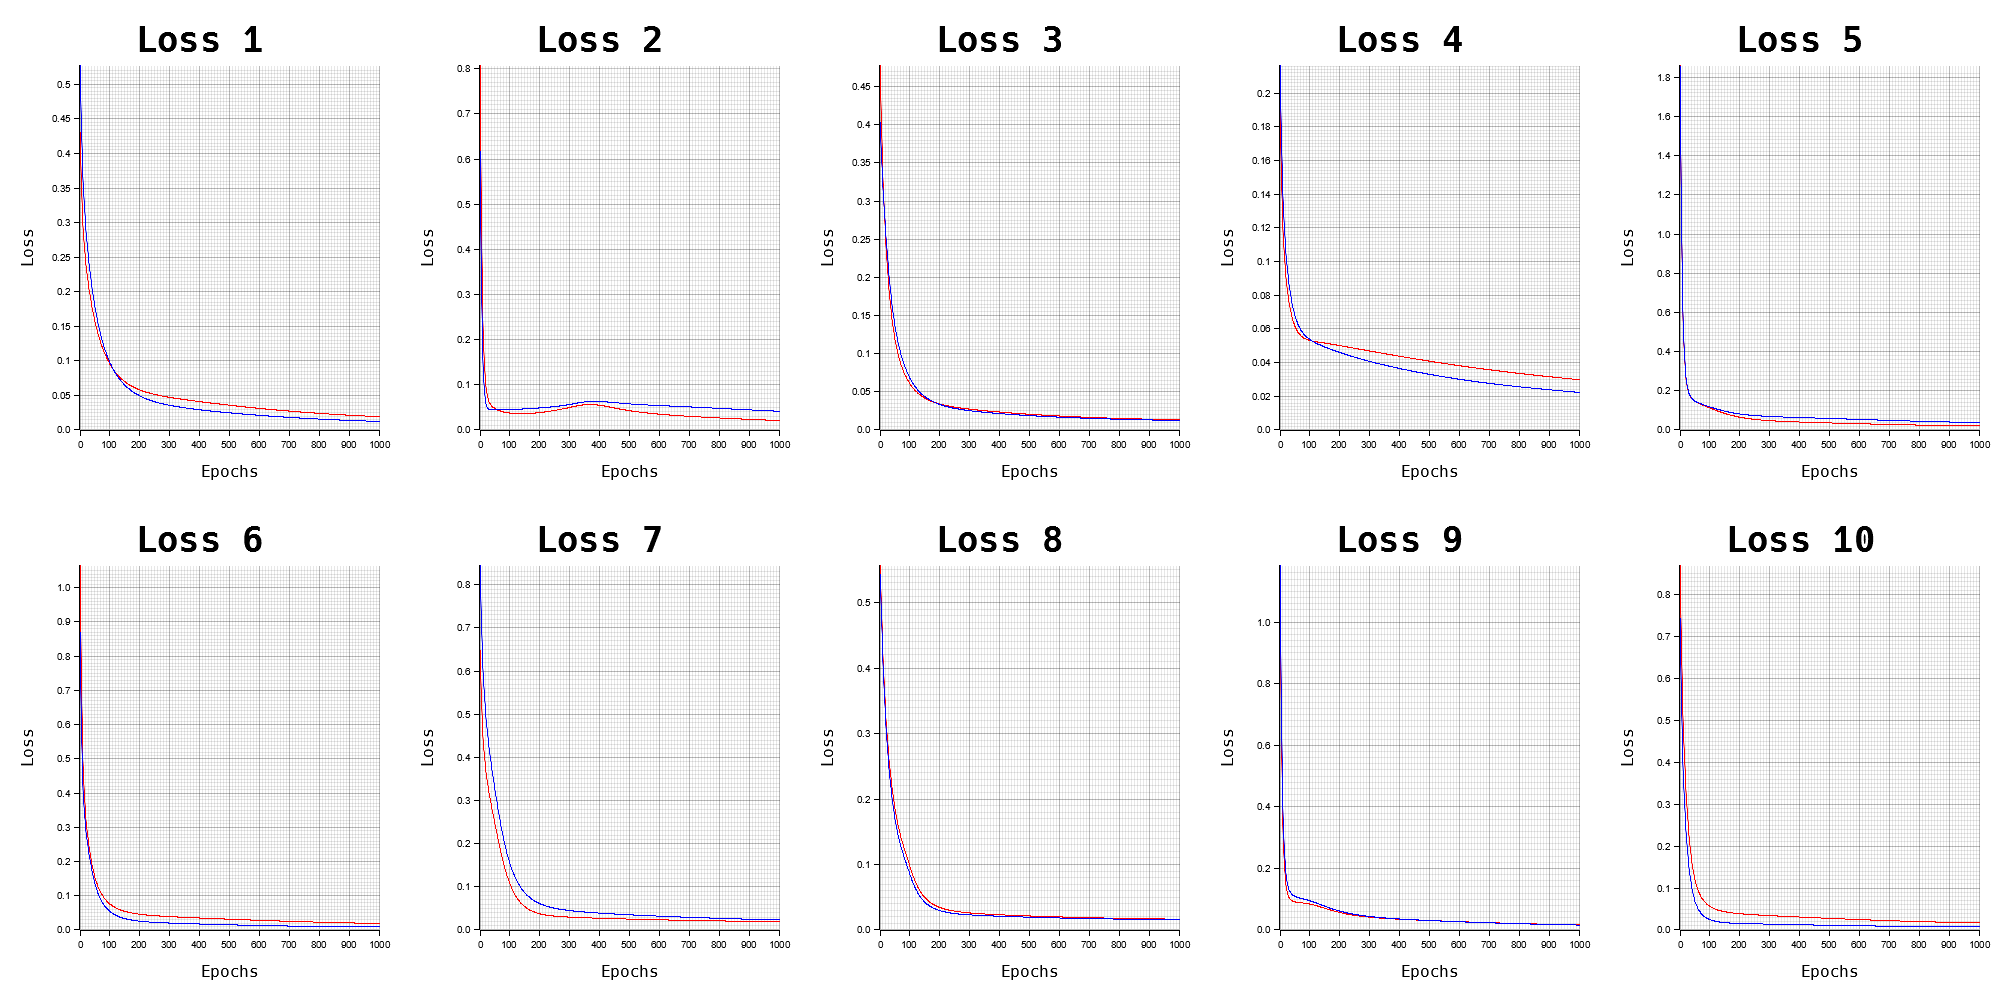
\includegraphics[width=\textwidth]{flood-8-4-1_3/loss}
		\caption{Each iteration training MSE (blue) and validation MSE (red) at each epoch.}
		\label{fig:4b}
	\end{subfigure}
	\caption{Training result of Flood-8-4-1 with smaller learning rate.}
	\label{fig:4}
\end{figure}
\FloatBarrier

\newpage
\subsection*{Flood-8-4-1 with no data preprocessing}
Same base model train with $lr = 0.01$ and $momentum = 0.01$ but 
it is the only model with no data preprocessing. The training process takes about $57$ seconds.
Below are the graphs we get from training this model. 
\begin{figure}[ht]
	\begin{subfigure}{\textwidth}
		\centering
		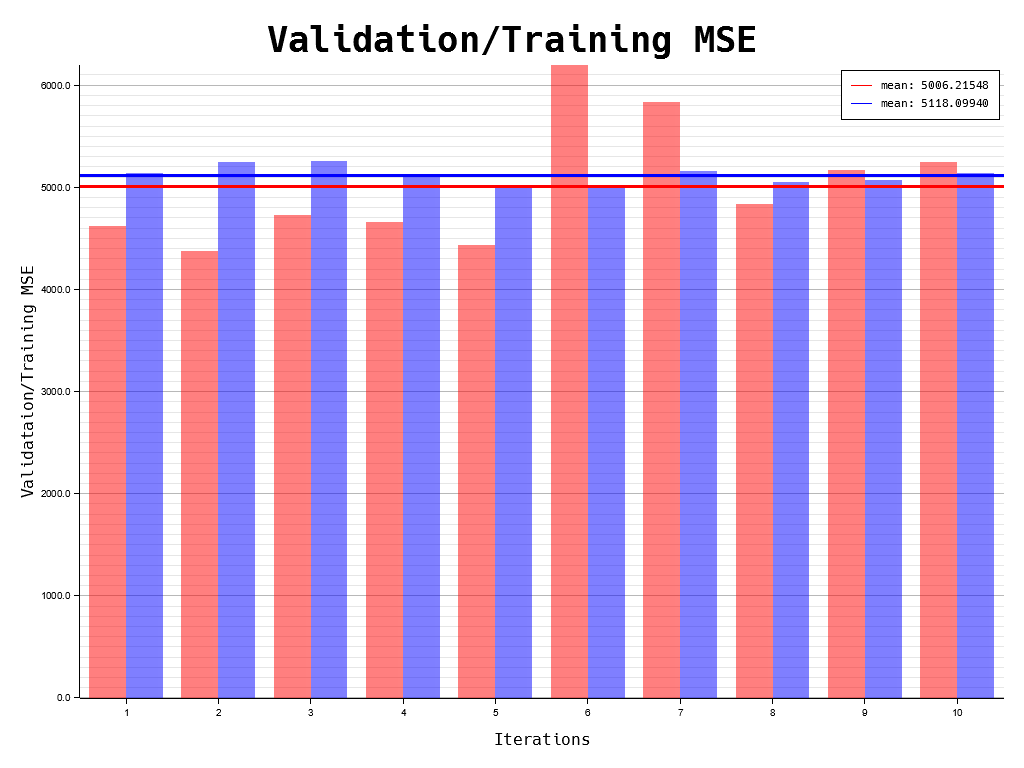
\includegraphics[scale=0.3]{flood-8-4-1_4/cv_l}
		\caption{Each iteration training (blue) and validation (red) RMSE at last epoch}
		\label{fig:5a}
	\end{subfigure}
	\begin{subfigure}{\textwidth}
		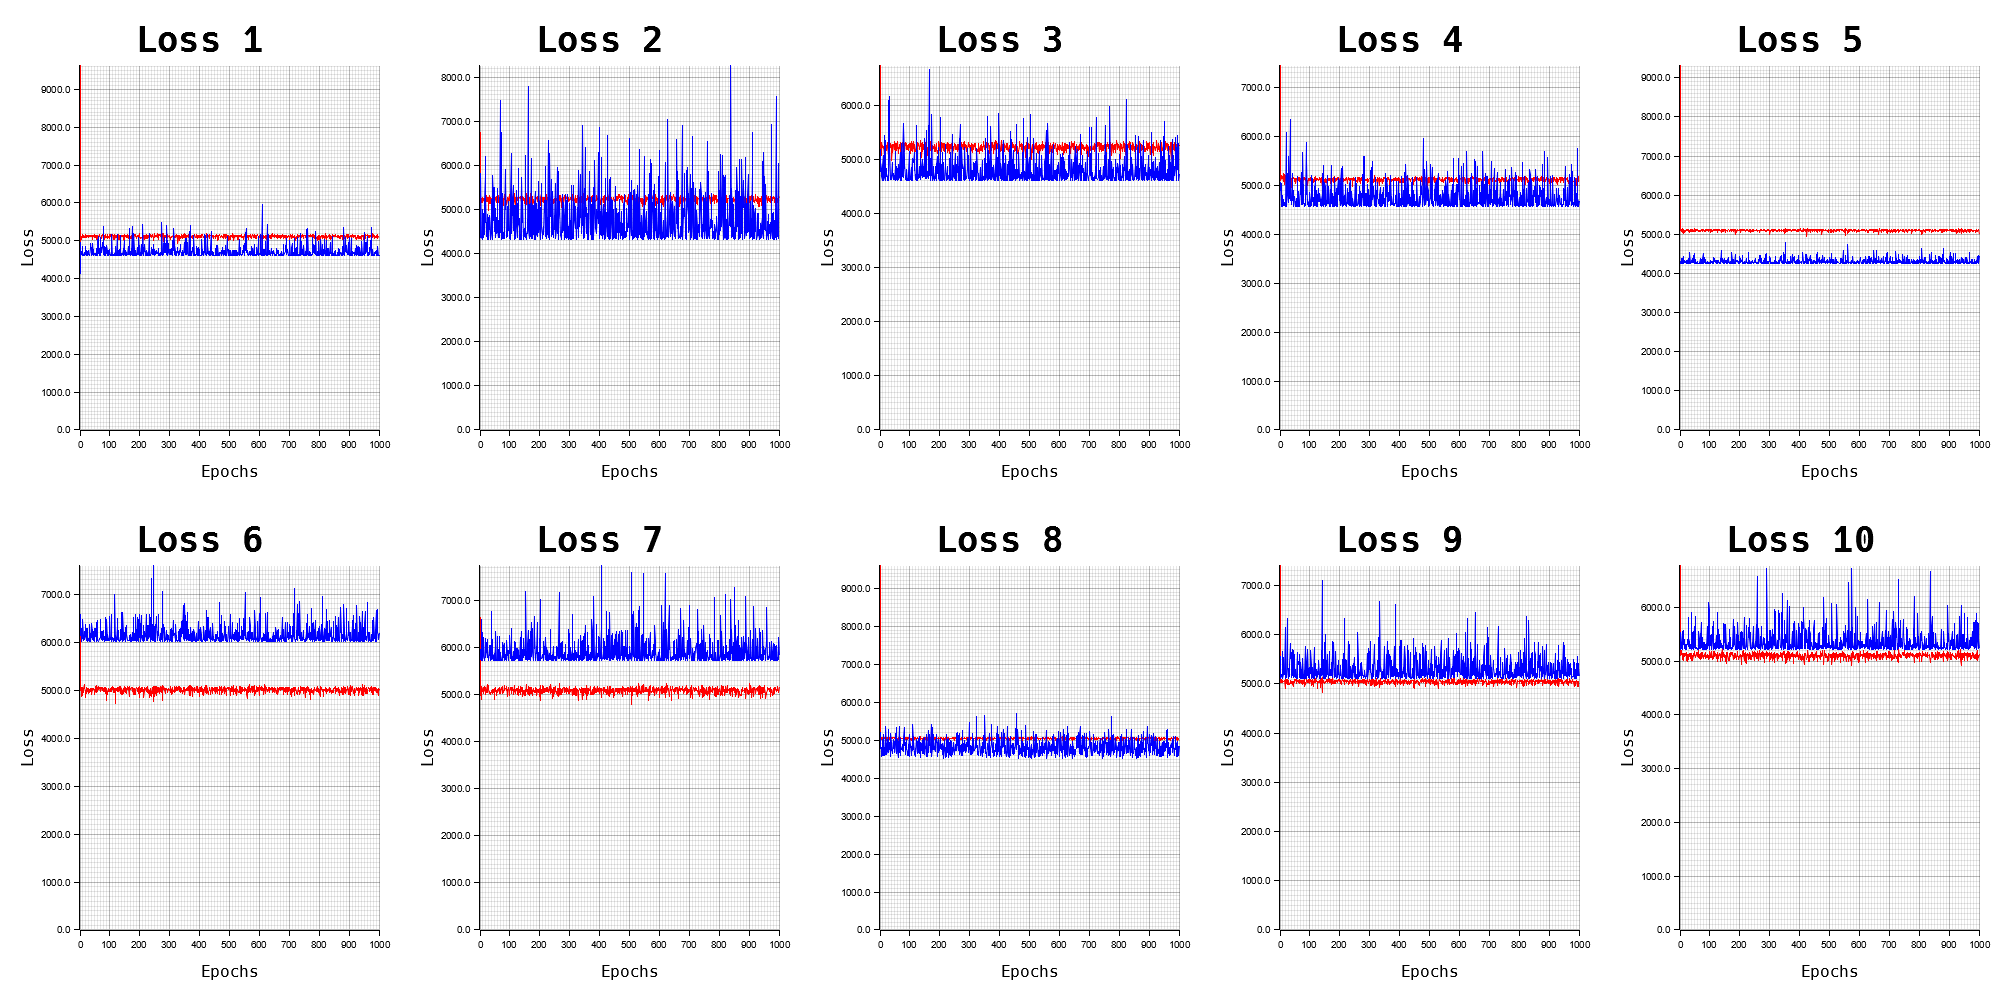
\includegraphics[width=\textwidth]{flood-8-4-1_4/loss}
		\caption{Each iteration training MSE (blue) and validation MSE (red) at each epoch.}
		\label{fig:5b}
	\end{subfigure}
	\caption{Training result of Flood-8-4-1 with no data preprocessing.}
	\label{fig:5}
\end{figure}
\FloatBarrier

\newpage
\subsubsection*{Flood-8-8-1}
Bigger model that contains 8 input nodes, 1 hidden layer with 8 nodes, and 1 output node train with $lr = 0.01$ and $momentum = 0.01$.
The training process takes about $105$ seconds.
Below are the graphs we get from training this model. 
\begin{figure}[ht]
	\begin{subfigure}{\textwidth}
		\centering
		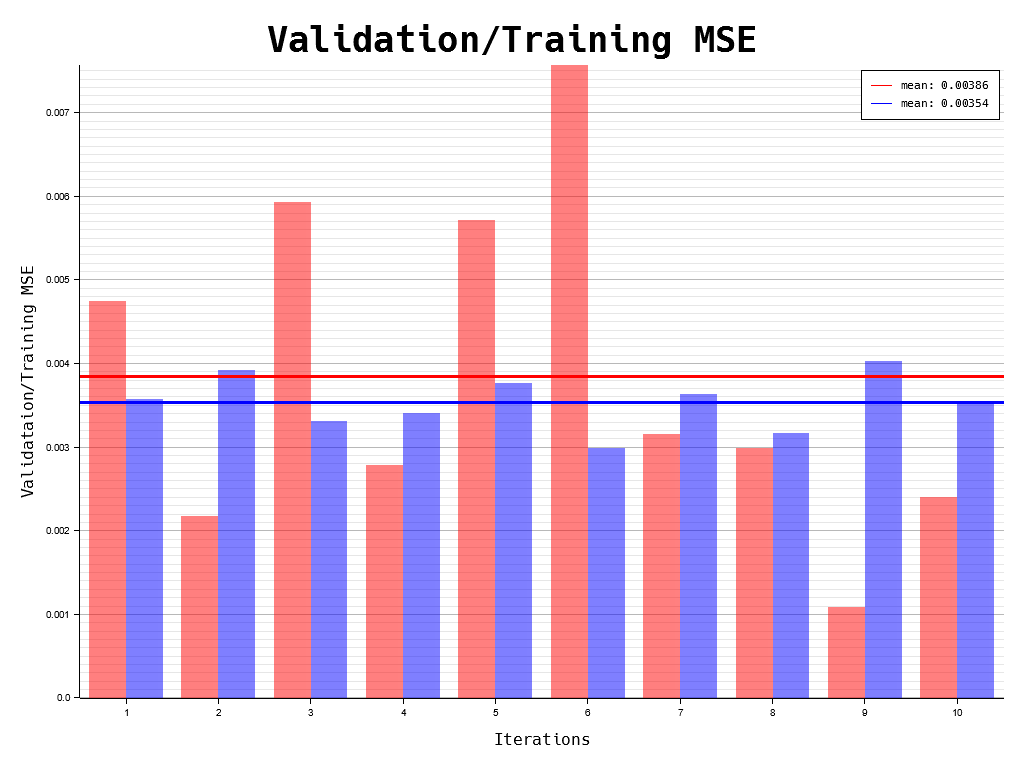
\includegraphics[scale=0.3]{flood-8-8-1/cv_l}
		\caption{Each iteration training (blue) and validation (red) RMSE at last epoch}
		\label{fig:6a}
	\end{subfigure}
	\begin{subfigure}{\textwidth}
		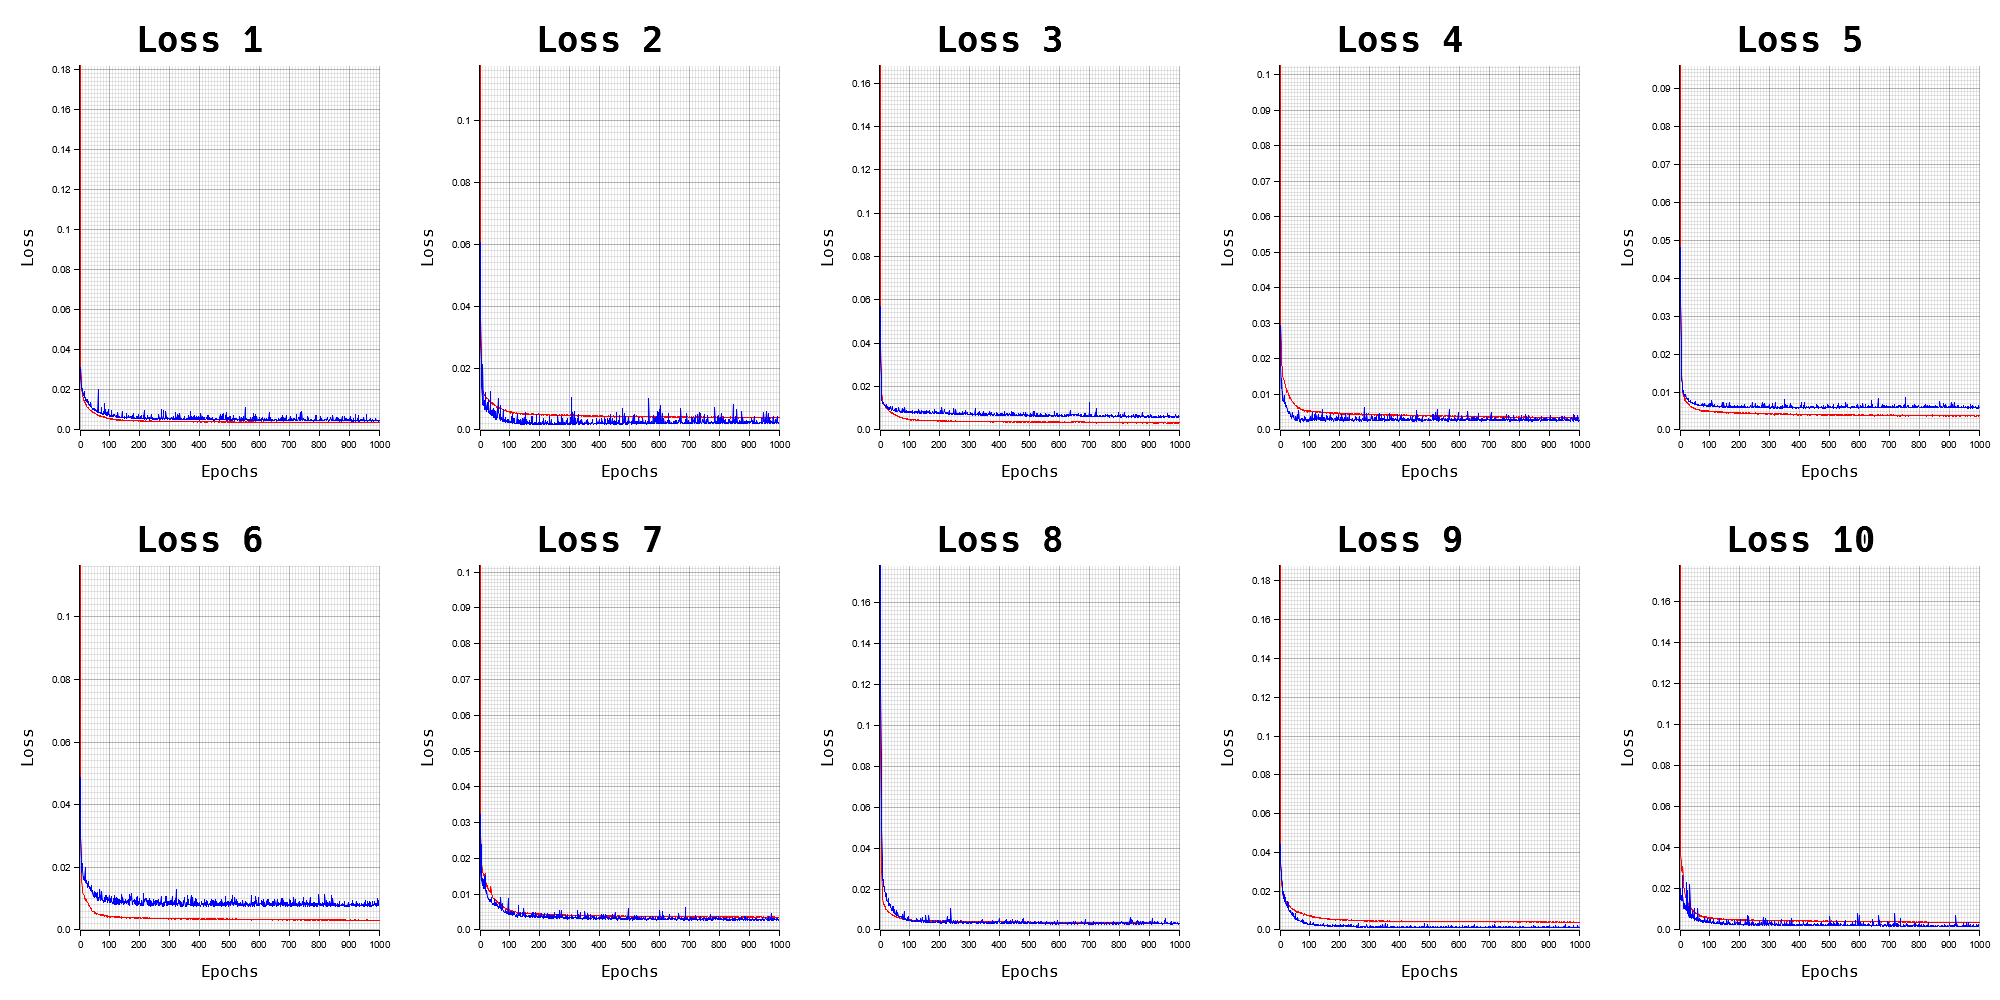
\includegraphics[width=\textwidth]{flood-8-8-1/loss}
		\caption{Each iteration training MSE (blue) and validation MSE (red) at each epoch.}
		\label{fig:6b}
	\end{subfigure}
	\caption{Training result of Flood-8-8-1.}
	\label{fig:6}
\end{figure}
\FloatBarrier


\newpage
\subsection*{Analysis}
From \cref*{table:1}, we can see that models with the same size will use around 
the same amount of training time, but with the bigger model, the training time 
gets longer. We can also see that Flood-8-4-1 with small learning rate 
is the worst in terms of validation set mean RMSE compare 
with other models that do data preprocessing, the model seems to be stuck at a certain gradient level 
(see \cref{fig:4b} the model is slowly converging but too slow). 
Surprisingly, the best performing model in terms of validation set mean
RMSE is the base model Flood-8-4-1 that has mean RMSE at $6.023 \times 10^{-2}$ 
not the bigger model Flood-8-8-1 that has more hidden nodes.

\begin{table}[htp]
	\centering
	\begin{tabular}{l S[table-format=3] S[table-format=4.3]}
		\toprule
        \multicolumn{1}{c}{Model} & {Training Time (seconds)} & {Validation Set Mean RMSE ($10^{-2}$)} \\
        \midrule
        Flood-8-4-1 & 56 & 6.023 \\
        Flood-8-4-1 with no momentum & 56 & 6.383 \\
        Flood-8-4-1 with small learniing rate & 56 & 14.400 \\
		Flood-8-4-1 with no data preprocessing & 57 & 7378.489 \\
        Flood-8-8-1 & 105 & 6.245 \\
        \bottomrule
    \end{tabular} 
    \caption{Training time and validation set mean RMSE 
		(red line on \cref{fig:2a}, \cref{fig:3a}, \cref{fig:4a},
		\cref{fig:5a}, and \cref{fig:6a} ) of each Flood model.}
	\label{table:1}
\end{table}
\FloatBarrier

We can also see a similar pattern on all of our Flood models in \cref{fig:2b}, \cref{fig:3b}
\cref{fig:4b}, and \cref{fig:6b} the MSE is decreasing very fast 
at the first 100 epochs and seems to be stuck at a certain level of MSE or 
very slow in MSE reduction. But, there is one model that does not follow this
pattern which is Flood-8-4-1 with no data preprocessing 
as we can see in \cref{fig:5b}, the training MSE seems to be flickering a lot
and there is no sign of the training MSE converging indicating that 
the model is struggling to learn with big error that comes 
from not standardized data e.g. we are training a model with not standardized data; the result from 
forward pass is $170$, the desired value is $150$, we'll get MSE $= (170 - 150)^{2} = 400$ 
compared with standardized data; imagine the training set $mean = 340$, 
$std = 120$ the desired value will be $\frac{(150 - mean)}{std} \approx -1.58$
and suppose that the result from forward pass will be $\frac{(170 - mean)}{std} \approx -1.42$,
we will get MSE $= (-1.42 -(-1.58))^{2} = 0.0256$ which is much smaller than not
standardized data MSE (note that there is no need for the result from forward pass to be exactly like that,
I use that conversion to only point out that in standardized data the MSE is much smaller).

\newpage
\section*{CrossPat Dataset}
\subsection*{Problem}
We want to predict the class (1 of possible 2 classes) that belongs
to our inputs (or features).

\begin{figure}[ht]
	\centering
	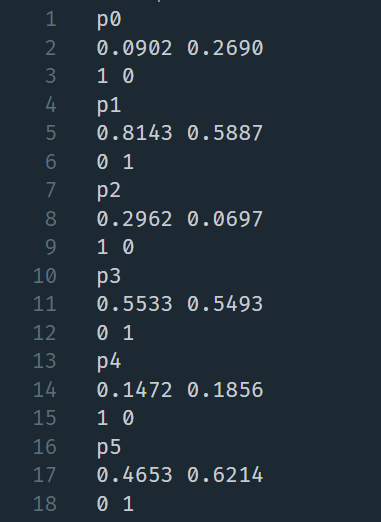
\includegraphics[scale=0.5]{cross_data}
	\caption{Examples of given data where p$x$ is an object and 
	the first line after it is its features, the second line is its class}
\end{figure}
\FloatBarrier

\subsection*{Parameters Setting}
\begin{itemize}
	\item All nodes use $sigmoid$ as an activation function.
	\item Weights are random number that is in range $[-1, 1]$
	\item Each layer's bias is $1$
	\item Use MSE (Mean Squared Error) as a loss function.
\end{itemize}

\subsection*{Training}
Use 10\% cross-validation with no data preprocessing, and train with SGD (Stochastic Gradient Descent) algorithm. Then, we train each cross-validation set for $5000$ epochs.

We will create one base model that should perform good enough 
and create a variations base on that model, that is train 
with no \emph{momentum}, train with smaller \emph{learning rate}, 
and add more layers or hidden nodes to see that if we introduce 
those variations, will the model perform better, converge faster, or have no improvement?

\subsection*{Training Result}
We use only 1 output node in all models because this is a binary classification task so we can just map a pair $(1, 0) \rightarrow 1$ and $(0, 1) \rightarrow 0$.
We then have a threshold at $0.5$ if output is more than $0.5$ then it is $1$ else it is $0$.
Accuracy is then calculated by using this equation $\frac{TP+TN}{TP+TN+FN+FP}$ where $TP, TN, FN, FP$ come from confusion matrix.
\subsubsection*{Cross-2-4-1}
Our base model with 2 input nodes, 1 hidden layer with 4 nodes, and 1 output node train with $lr = 0.01$ and $momentum = 0.01$. 
The training process takes about 122 seconds..
\subsubsection*{Cross-2-4-1 with no momentum}
Same base model train with $lr = 0.01$ and $momentum = 0.0$.
The training process takes about 122 seconds.
\subsubsection*{Cross-2-4-1 with smaller learning rate}
Same base model train with $lr = 0.0001$ and $momentum = 0.01$.
The training process takes about 124 seconds.
\subsubsection*{Cross-2-8-1}
Bigger model that contains 2 input nodes, 1 hidden layer with 4 nodes, and 1 output node train with $lr = 0.01$ and $momentum = 0.01$.
The training process takes about 230 seconds.

\begin{figure}[ht]
	\begin{subfigure}{\textwidth}
		\centering
		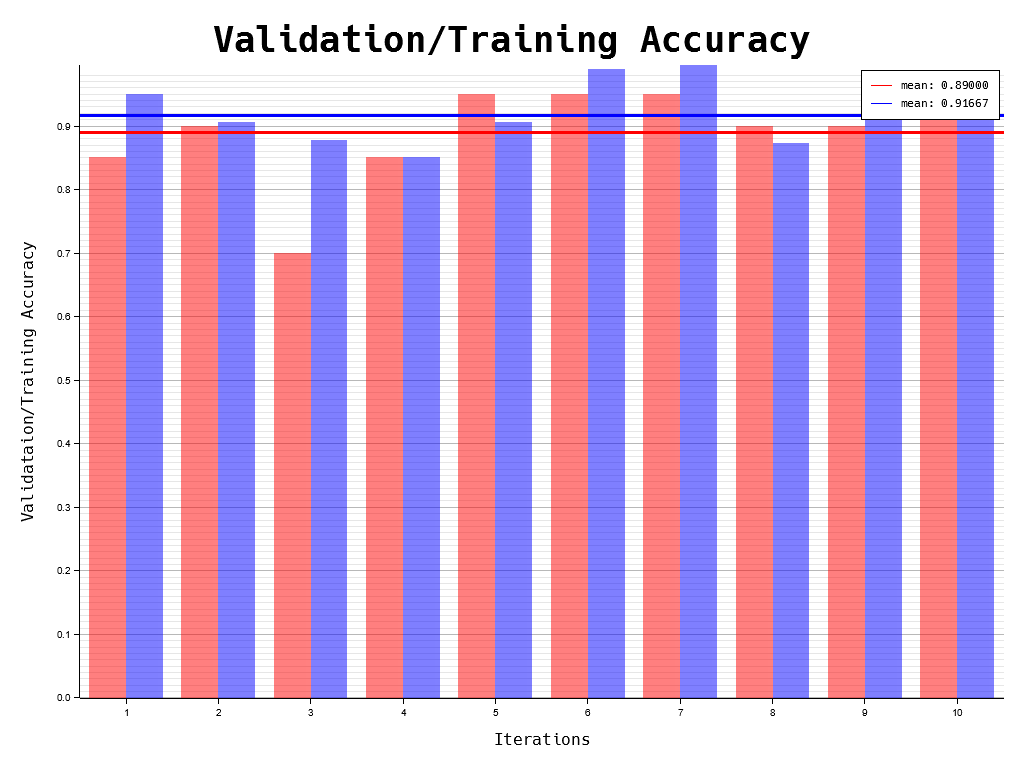
\includegraphics[width=0.5\textwidth]{cross-2-4-1/acc}
		\caption{Each iteration training (blue) and validation (red) set accuracy at last epoch}
		\label{fig:7a}
	\end{subfigure}
	\begin{subfigure}{\textwidth}
		\centering
		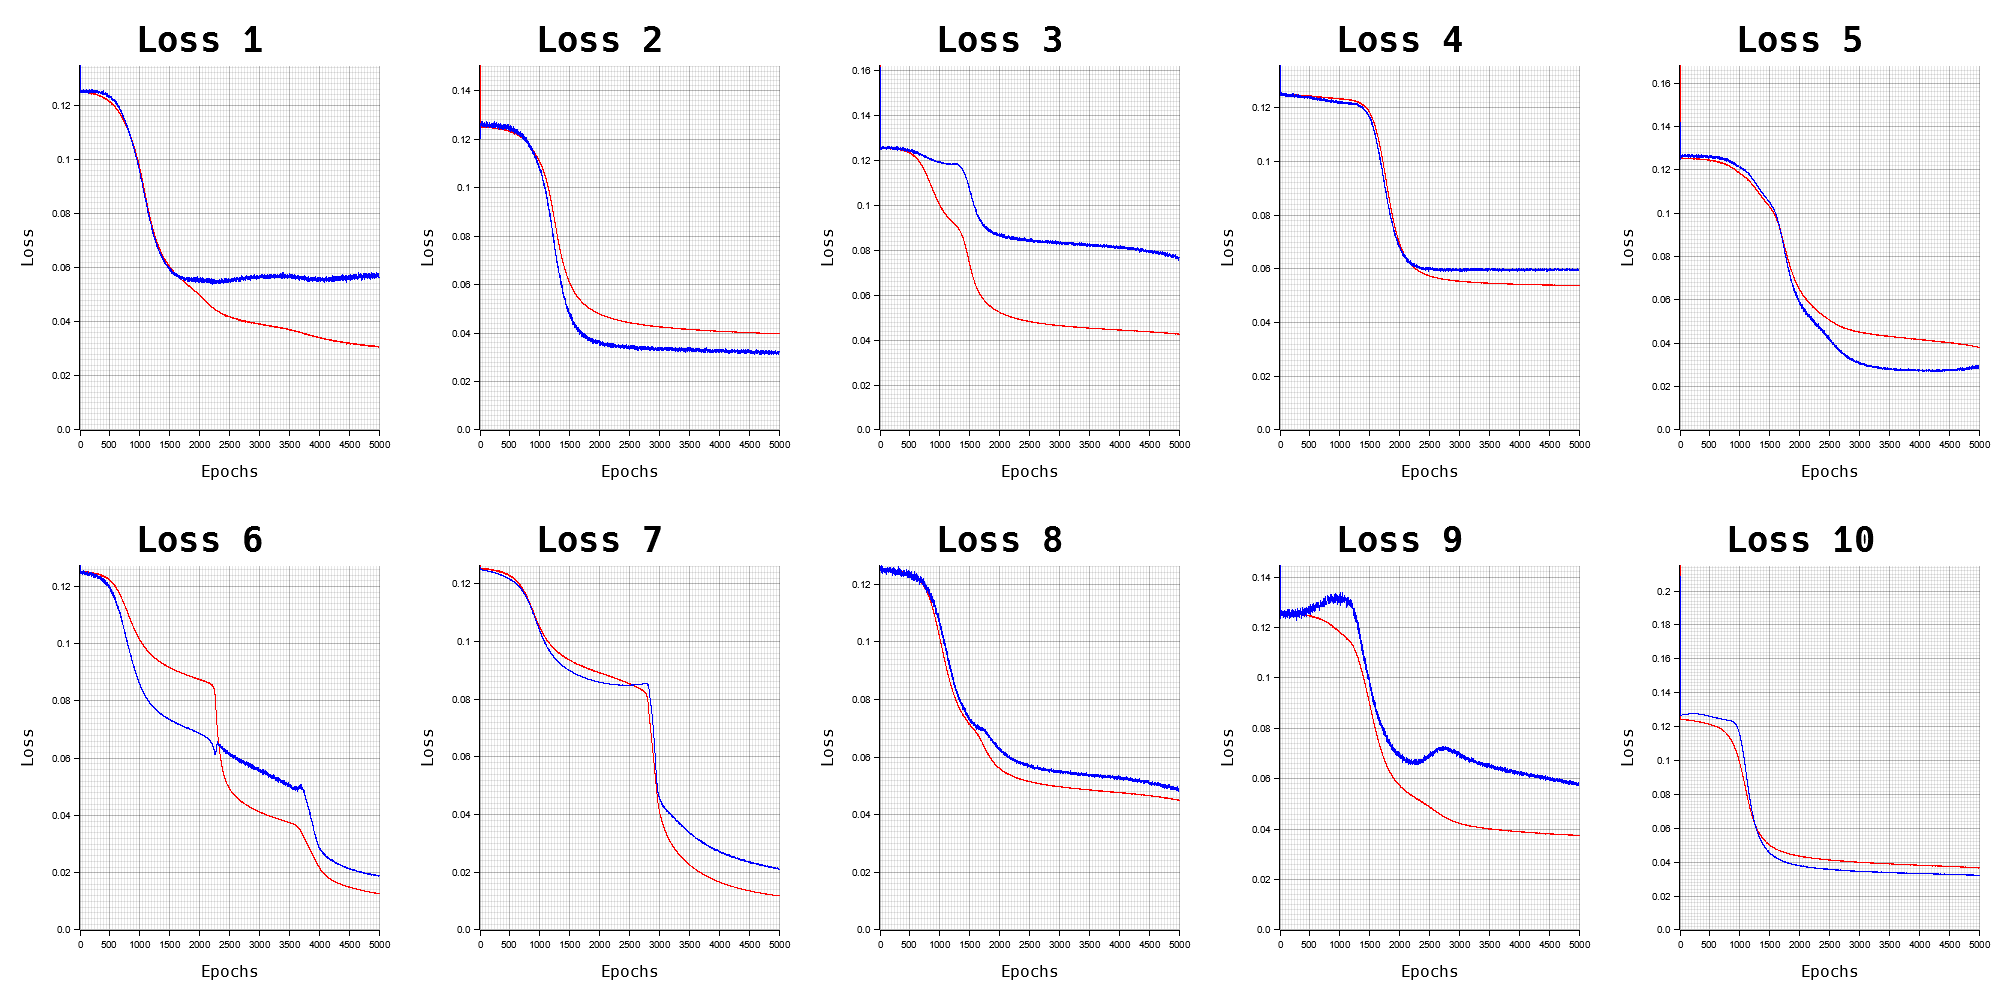
\includegraphics[width=0.9\textwidth]{cross-2-4-1/loss}
		\caption{Each iteration training MSE (blue) and validation MSE (red) at each epoch.}
		\label{fig:7b}
	\end{subfigure}
	\begin{subfigure}{\textwidth}
		\centering
		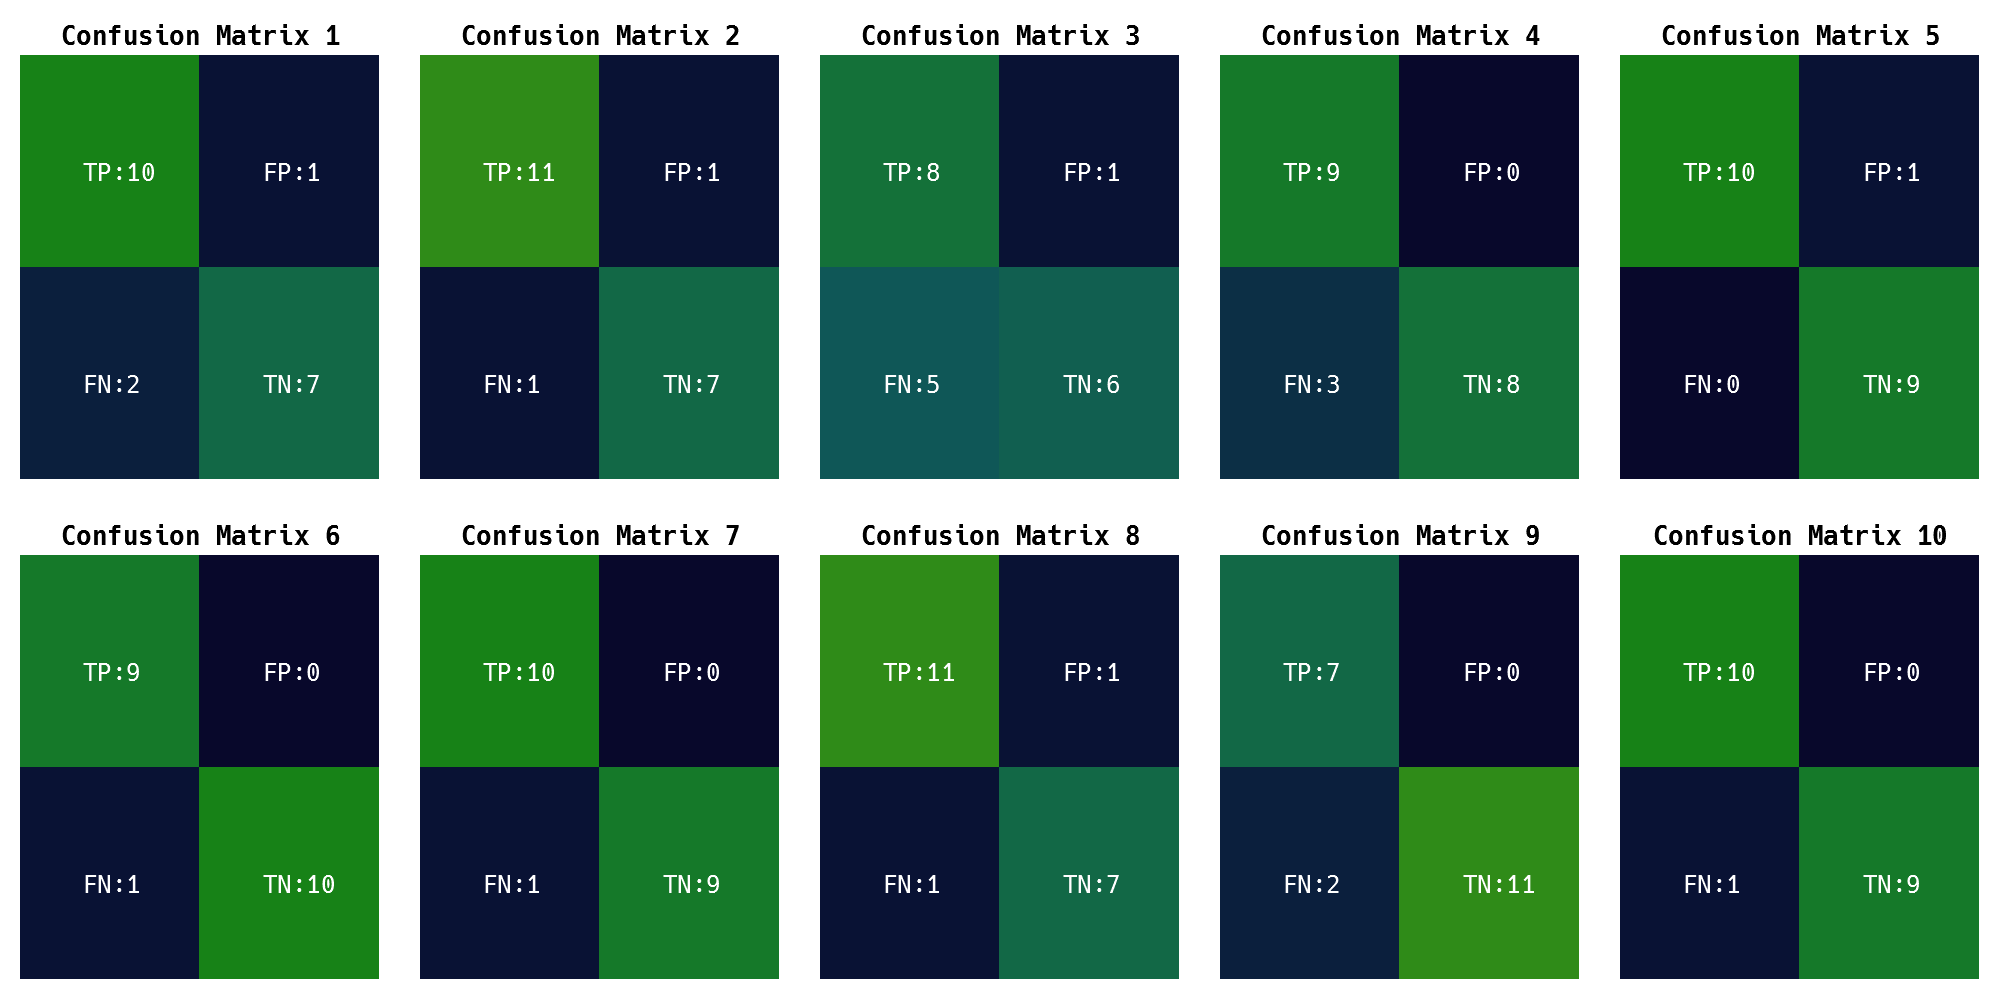
\includegraphics[width=0.9\textwidth]{cross-2-4-1/confusion_matrix}
		\caption{Each iterations validation set confusion matrix where y-axis is an actual class $1, 0$ top to bottom and x-axis is predicted class $1, 0$ left to right.}
		\label{fig:7c}
	\end{subfigure}
	\caption{Training result of Cross-2-4-1.}
	\label{fig:7}
\end{figure}
\FloatBarrier

\begin{figure}[ht]
	\begin{subfigure}{\textwidth}
		\centering
		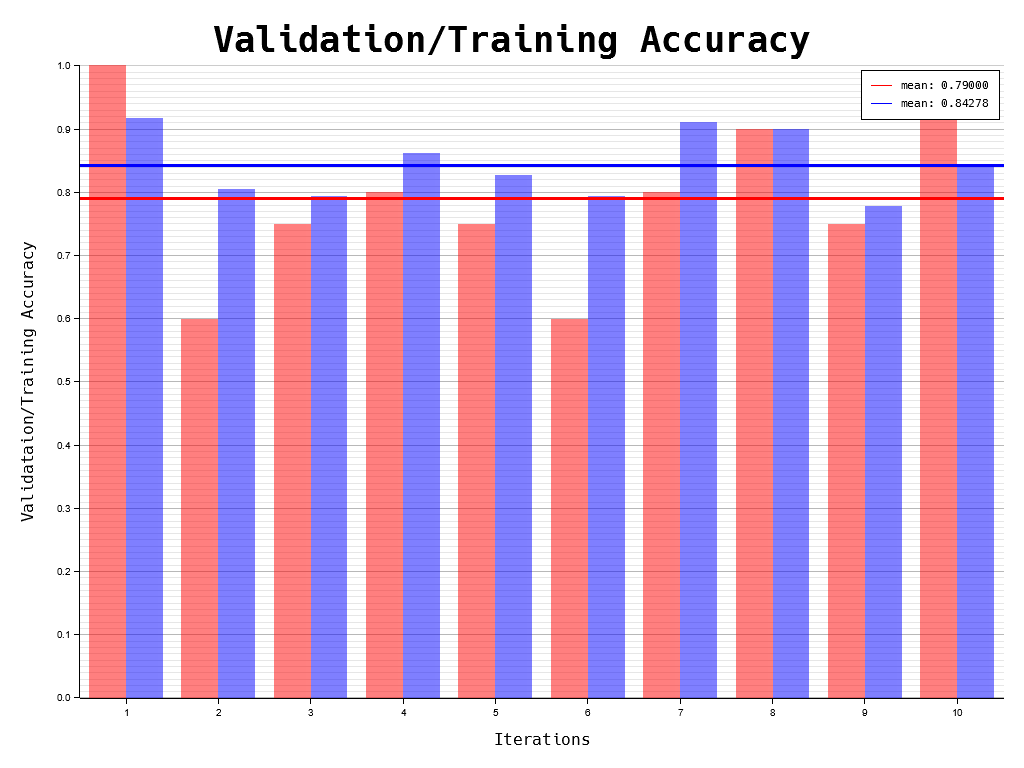
\includegraphics[width=0.5\textwidth]{cross-2-4-1_2/acc}
		\caption{Each iteration training (blue) and validation (red) set accuracy at last epoch}
		\label{fig:8a}
	\end{subfigure}
	\begin{subfigure}{\textwidth}
		\centering
		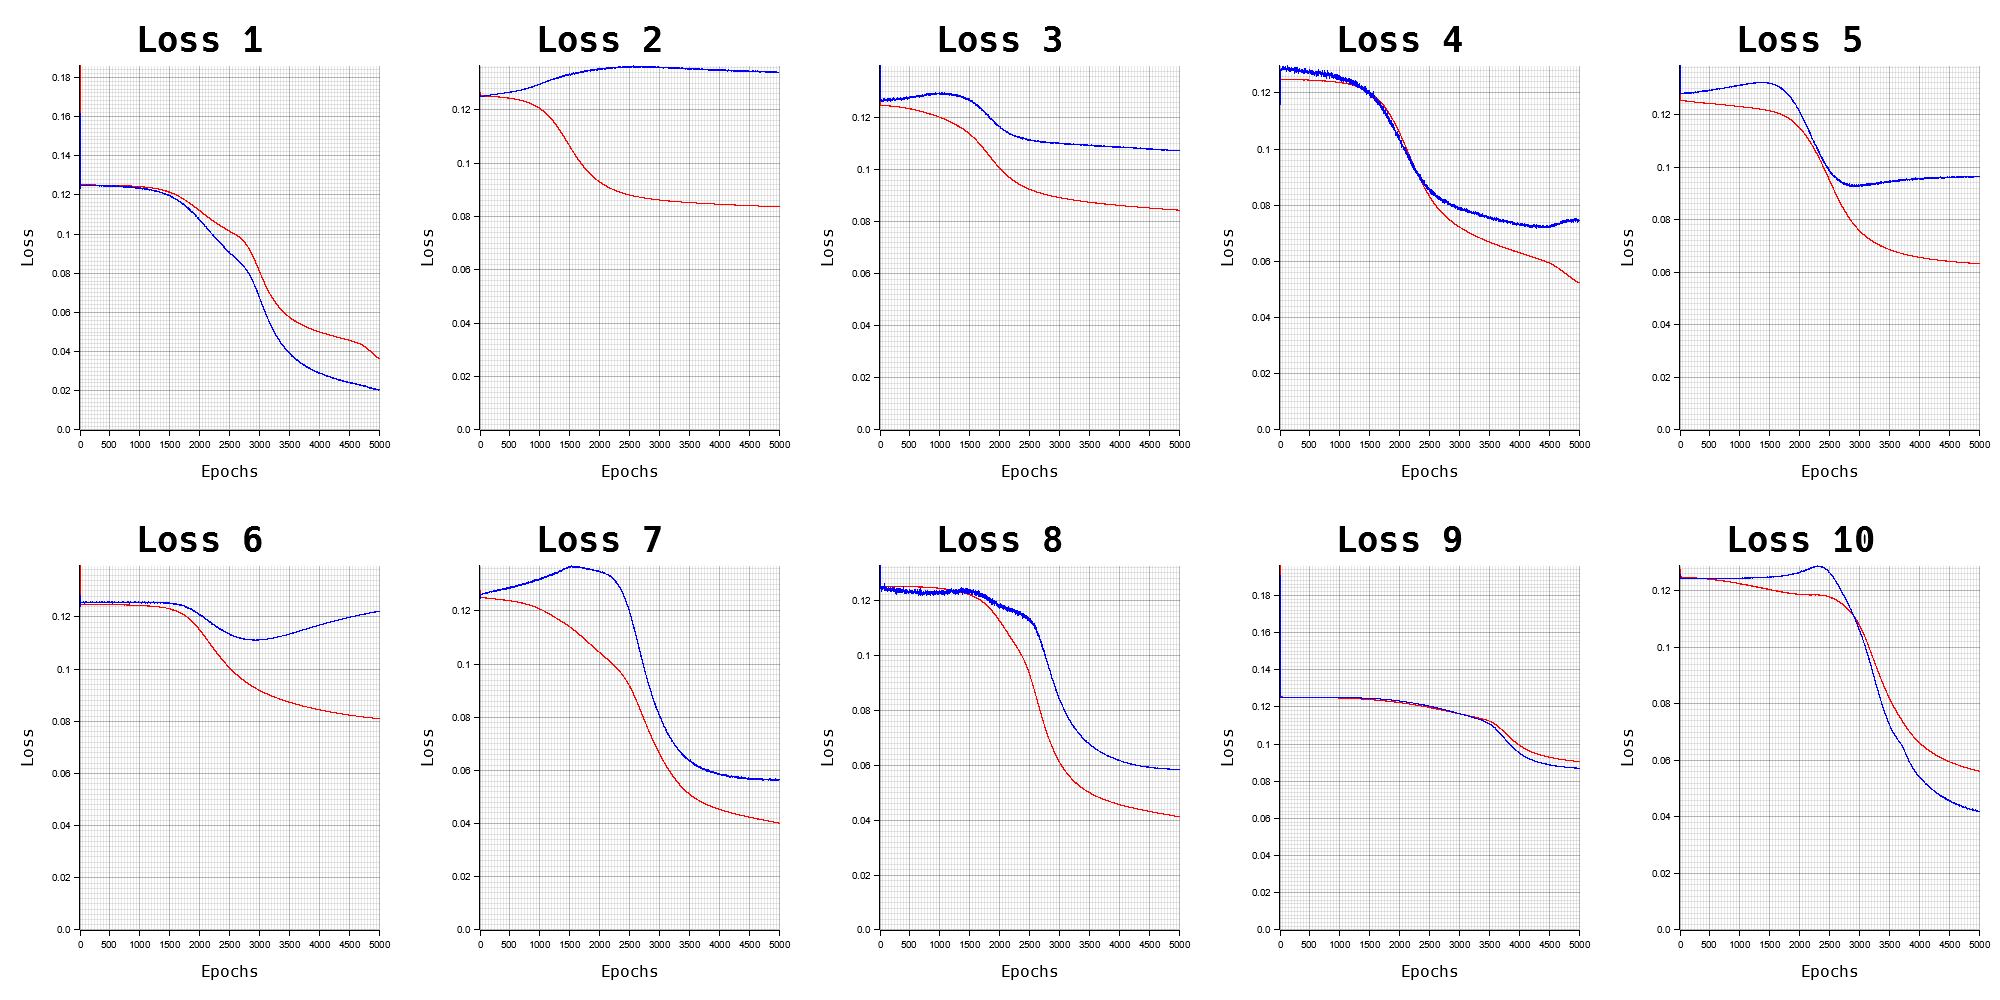
\includegraphics[width=0.9\textwidth]{cross-2-4-1_2/loss}
		\caption{Each iteration training MSE (blue) and validation MSE (red) at each epoch.}
		\label{fig:8b}
	\end{subfigure}
	\begin{subfigure}{\textwidth}
		\centering
		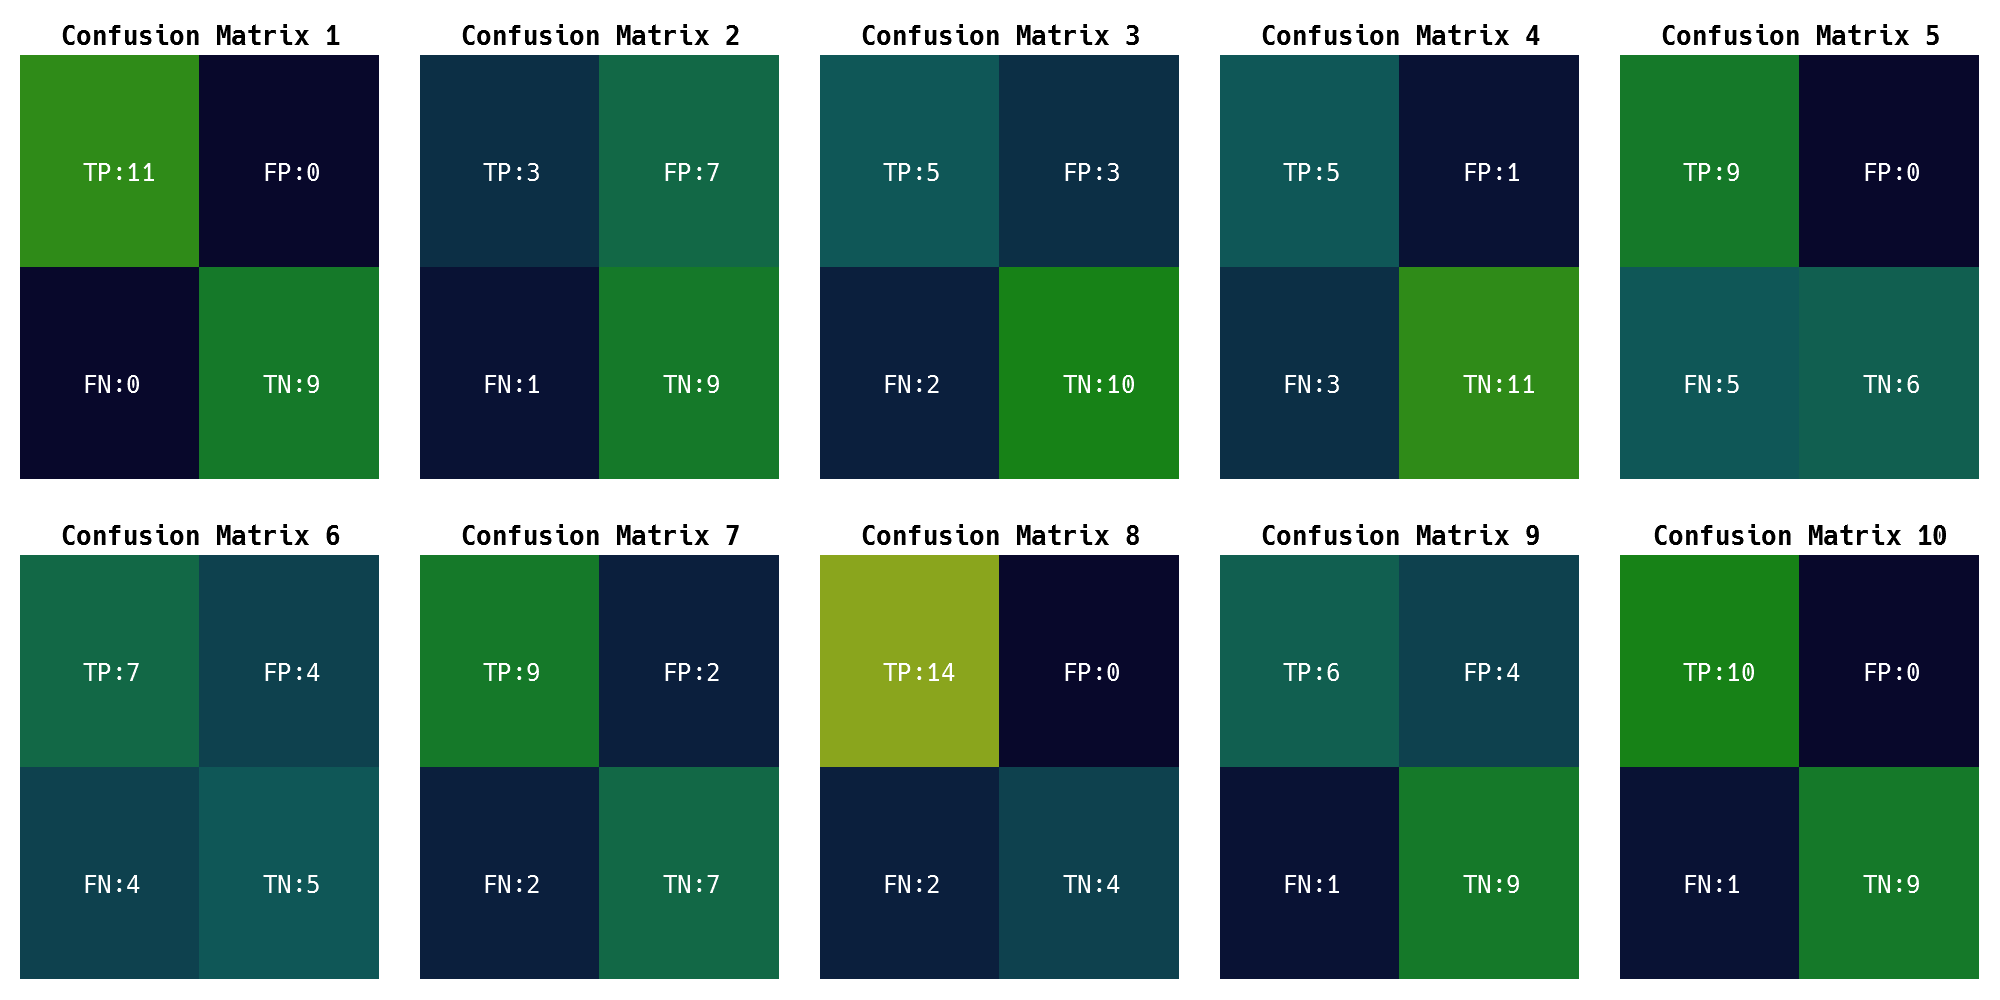
\includegraphics[width=0.9\textwidth]{cross-2-4-1_2/confusion_matrix}
		\caption{Each iterations validation set confusion matrix where y-axis is an actual class $1, 0$ top to bottom and x-axis is predicted class $1, 0$ left to right.}
		\label{fig:8c}
	\end{subfigure}
	\caption{Training result of Cross-2-4-1 with no momentum.}
	\label{fig:8}
\end{figure}
\FloatBarrier

\begin{figure}[ht]
	\begin{subfigure}{\textwidth}
		\centering
		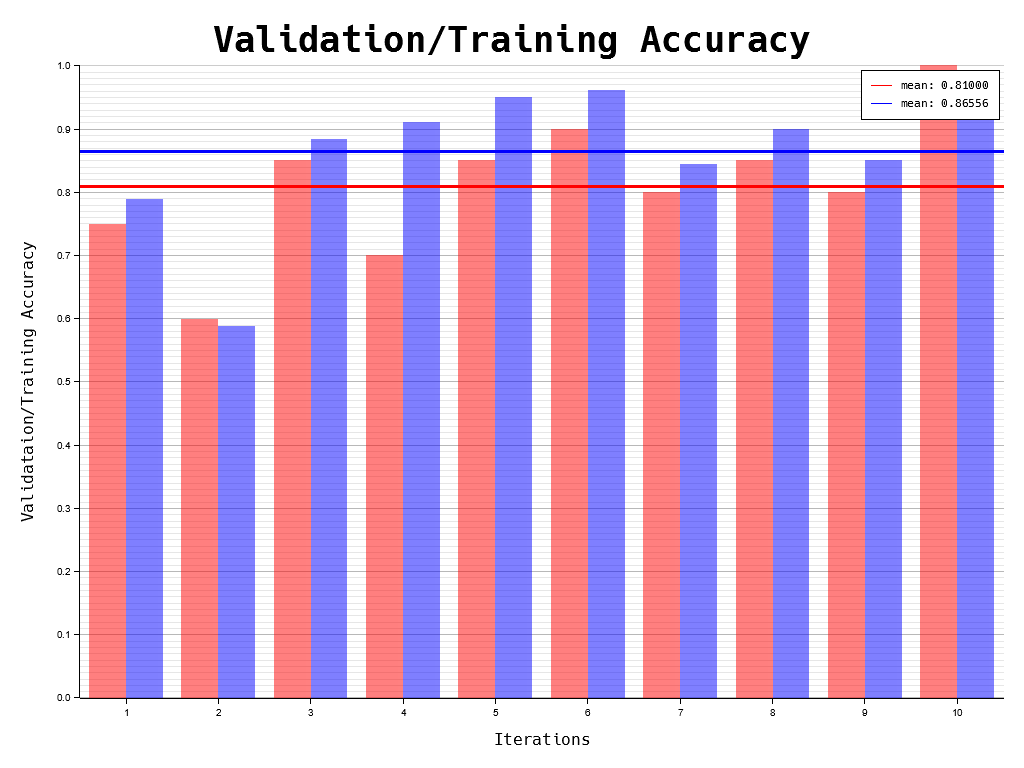
\includegraphics[width=0.5\textwidth]{cross-2-4-1_3/acc}
		\caption{Each iteration training (blue) and validation (red) set accuracy at last epoch}
		\label{fig:9a}
	\end{subfigure}
	\begin{subfigure}{\textwidth}
		\centering
		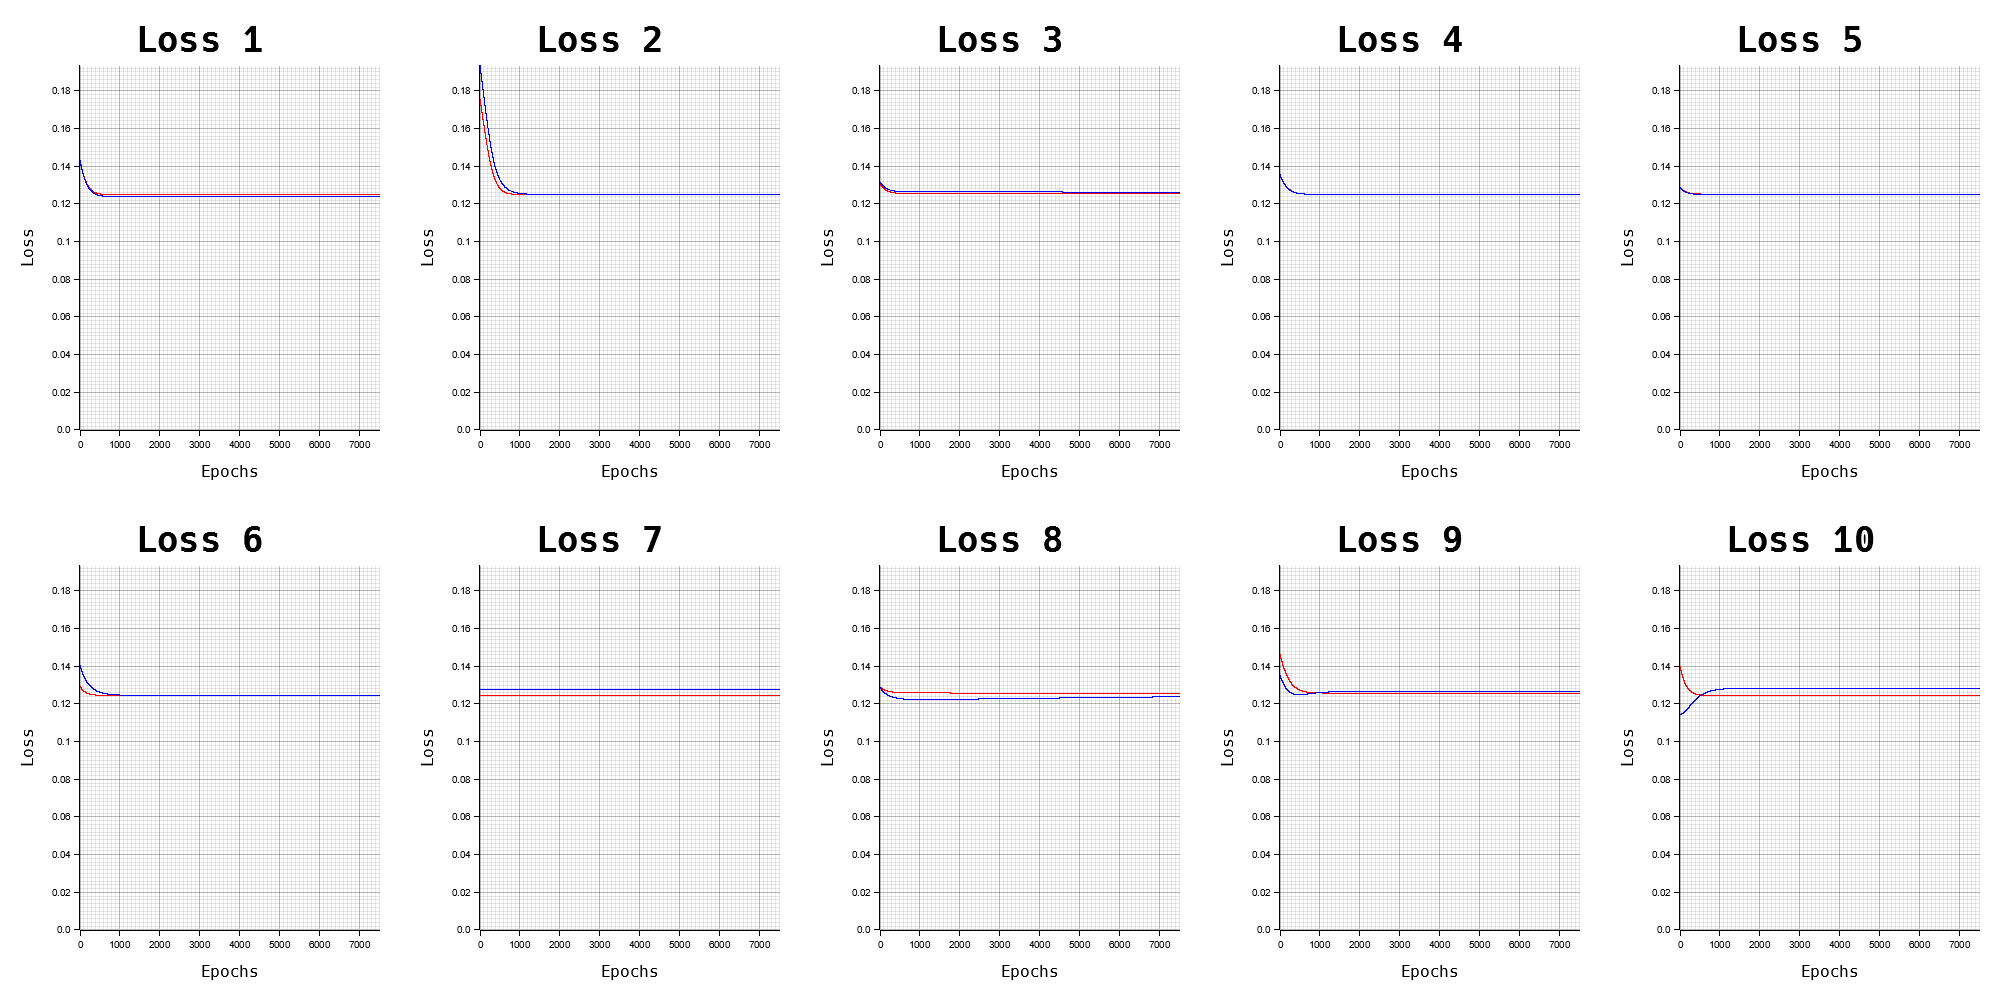
\includegraphics[width=0.9\textwidth]{cross-2-4-1_3/loss}
		\caption{Each iteration training MSE (blue) and validation MSE (red) at each epoch.}
		\label{fig:9b}
	\end{subfigure}
	\begin{subfigure}{\textwidth}
		\centering
		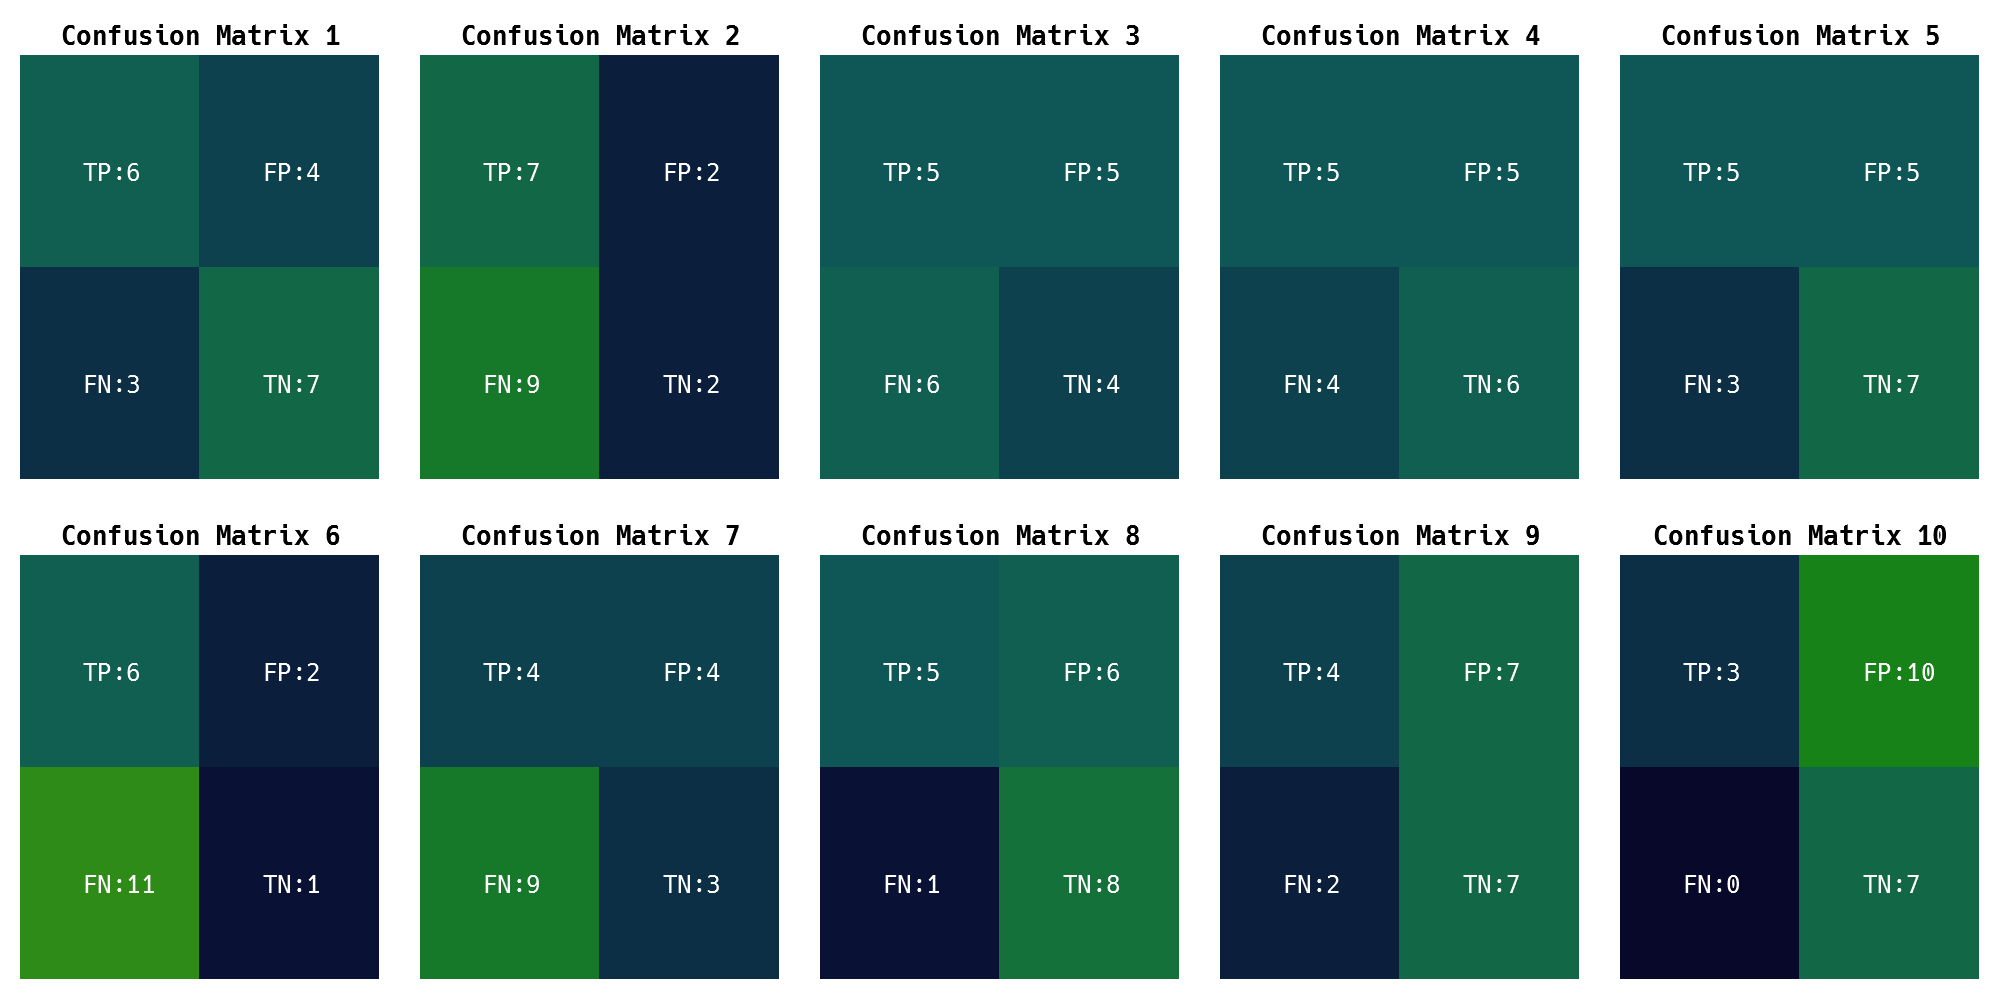
\includegraphics[width=0.9\textwidth]{cross-2-4-1_3/confusion_matrix}
		\caption{Each iterations validation set confusion matrix where y-axis is an actual class $1, 0$ top to bottom and x-axis is predicted class $1, 0$ left to right.}
		\label{fig:9c}
	\end{subfigure}
	\caption{Training result of Cross-2-4-1 with smaller learning rate.}
	\label{fig:9}
\end{figure}
\FloatBarrier

\begin{figure}[ht]
	\begin{subfigure}{\textwidth}
		\centering
		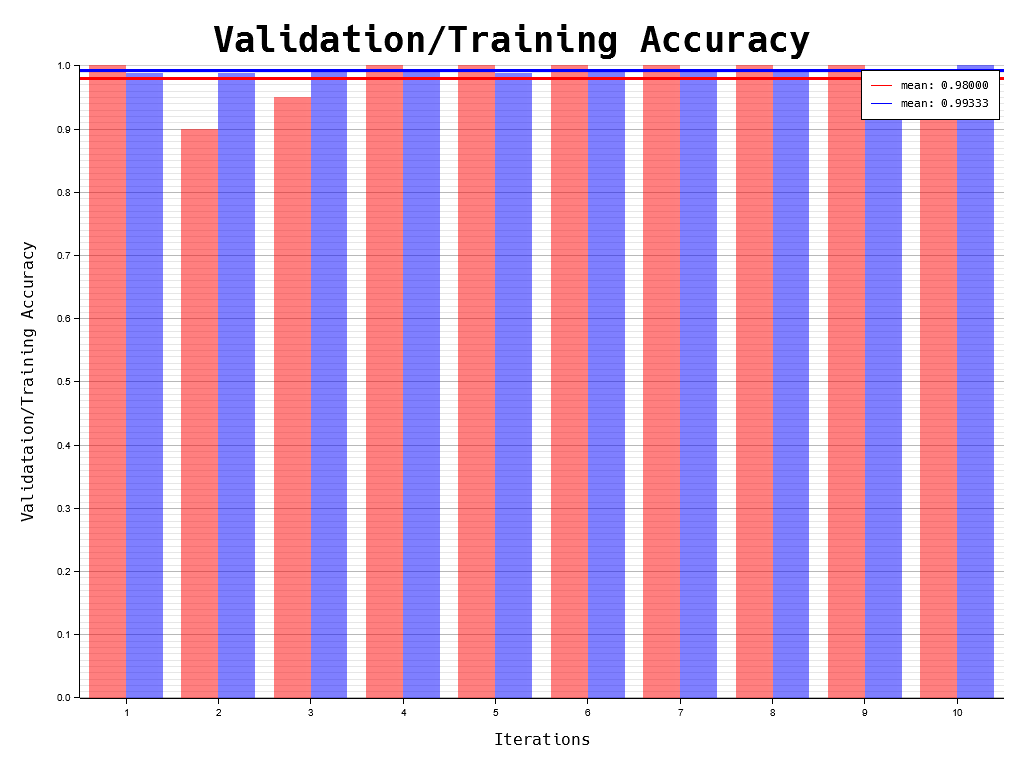
\includegraphics[width=0.5\textwidth]{cross-2-8-1/acc}
		\caption{Each iteration training (blue) and validation (red) set accuracy at last epoch}
		\label{fig:10a}
	\end{subfigure}
	\begin{subfigure}{\textwidth}
		\centering
		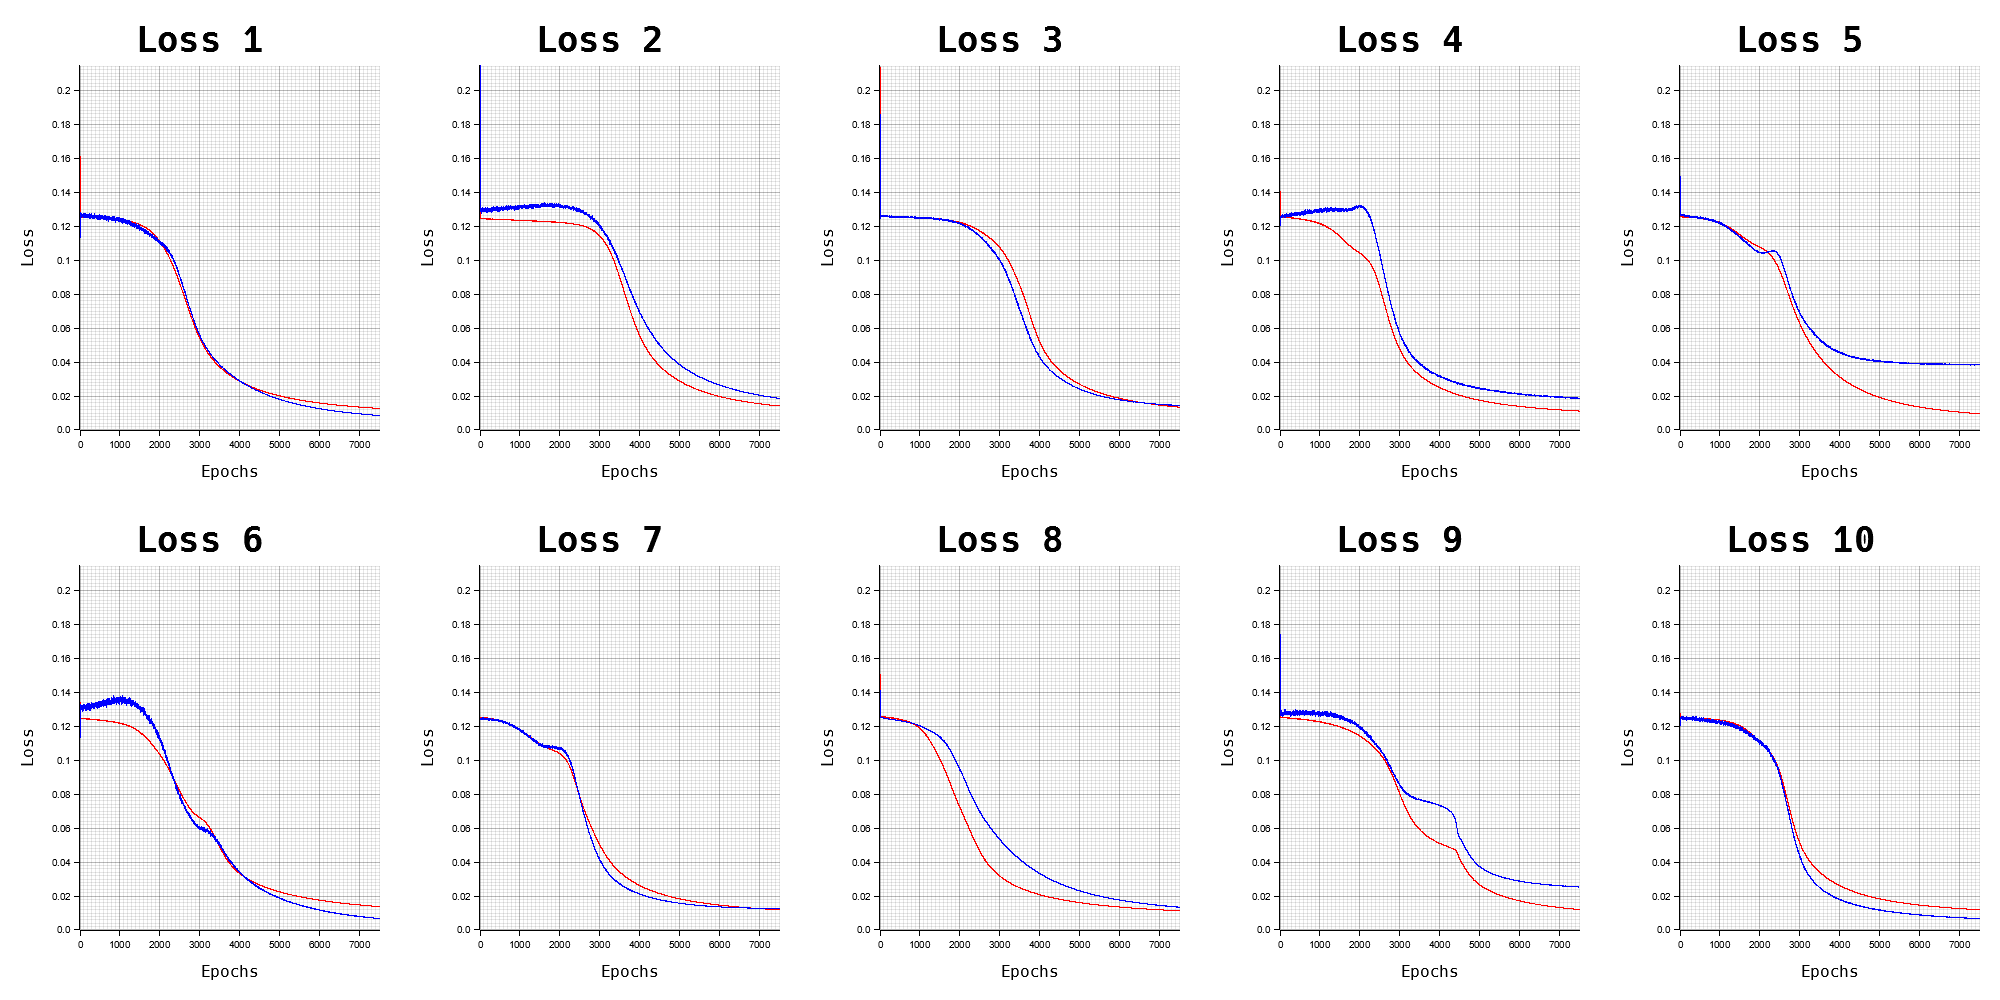
\includegraphics[width=0.9\textwidth]{cross-2-8-1/loss}
		\caption{Each iteration training MSE (blue) and validation MSE (red) at each epoch.}
		\label{fig:10b}
	\end{subfigure}
	\begin{subfigure}{\textwidth}
		\centering
		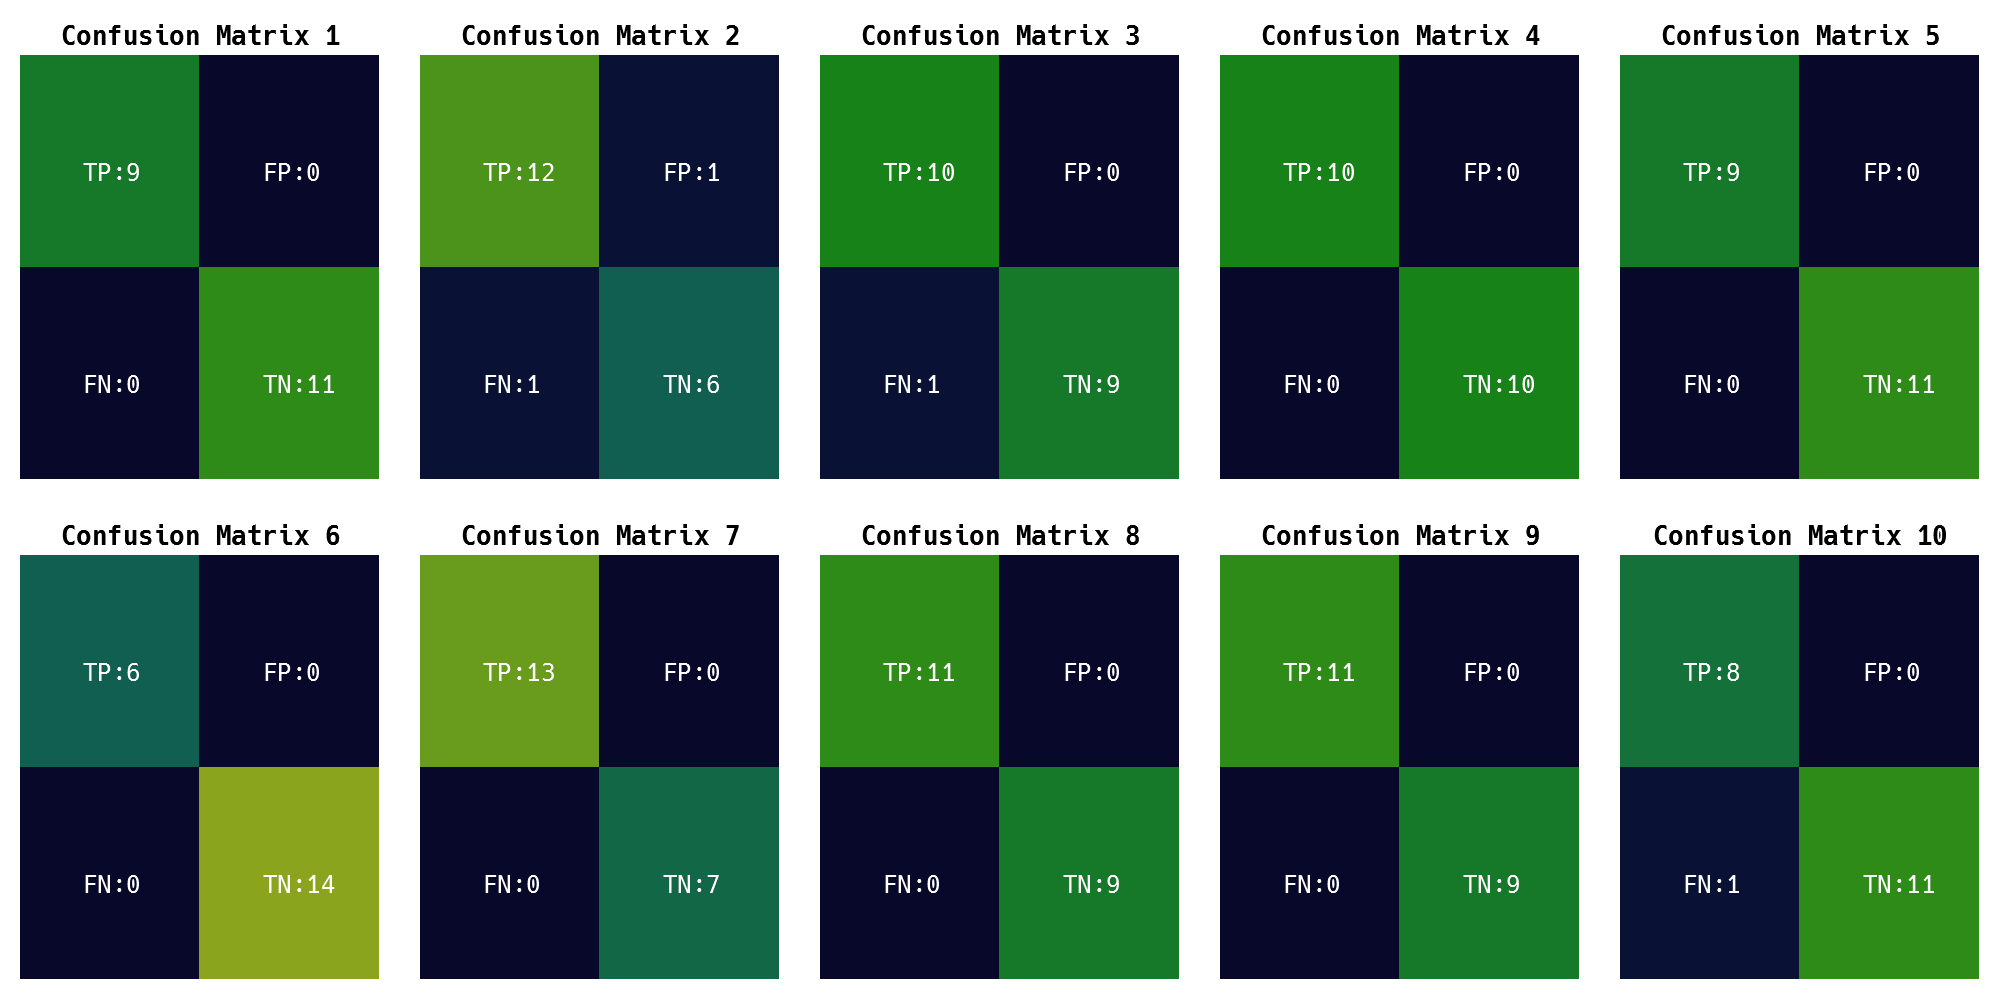
\includegraphics[width=0.9\textwidth]{cross-2-8-1/confusion_matrix}
		\caption{Each iterations validation set confusion matrix where y-axis is an actual class $1, 0$ top to bottom and x-axis is predicted class $1, 0$ left to right.}
		\label{fig:10c}
	\end{subfigure}
	\caption{Training result of Cross-2-8-1.}
	\label{fig:10}
\end{figure}
\FloatBarrier

\subsection*{Analysis}
From \cref*{table:2}, we can see that all Cross-2-4-1 models used around the 
same amount of training time but only the base model is performing okay in terms of
validation set mean accuracy. And the biggest model Cross-2-8-1 is performing much better than others at $98$\%
validation set mean accuracy but the training time used is also around 2 times other models training time.   

\begin{table}[htp]
	\centering
	\begin{tabular}{l S[table-format=3] S[table-format=2]}
		\toprule
        \multicolumn{1}{c}{Model} & {Training Time (seconds)} & {Validation Set Mean Accuracy (\%)} \\
        \midrule
        Cross-2-4-1 & 122 & 89 \\
        Cross-2-4-1 with no momentum & 122 & 79 \\
        Cross-2-4-1 with small learniing rate & 124 & 81 \\
        Cross-2-8-1 & 230 & 98 \\
        \bottomrule
    \end{tabular} 
	\caption{Training time and validation set mean accuracy (red line on 
		\cref{fig:7a}, \cref{fig:8a}, \cref{fig:9a}, and \cref{fig:10}) of each Cross model.}
	\label{table:2}
\end{table}

From \cref{fig:10b}, we can also see that Cross-2-8-1 training is going smoother 
with a steady decrease in MSE compared with other models as we can see in \cref{fig:7b}, \cref{fig:8b}, and 
\cref{fig:9b} the graphs overall seem to go down and stop at a certain level indicating that
the model stop learning. Confusion matrix of Cross-2-8-1 from \cref{fig:10c} also,
show that the error is not biased to one specific class indicating that the model learned
about the 2 classes equally. On the other hand, the confusion matrix of all Cross-2-4-1 models
specifically in \cref{fig:8c} and \cref{fig:9c} we can see that there're a big number
of FP and FN and in some iteration the error is biased to one of FP or FN.

\section*{Summary}
From both problems, we have learned that an MLP model can solve these problems 
and the performance of the model is dependent on parameters that we can set 
for the model such as learning rate, momentum, and size of the model as we can see
in the above experimenting result. And, in some datasets, there is a need for data 
preprocessing so that the model does not struggle to learn with that dataset as we can see in \nameref{section:1}.  

\end{document}
